\documentclass[10pt,a4paper]{article}

%%%%%%%%%%%%%%%%%%%%%%%%%%%
% MODIFY:

\newcommand{\authorA}{ALEX PASQUALI (03754113)}
\newcommand{\authorB}{NICOLA GUGOLE (03753996)}
\newcommand{\groupNumber}{A} % - YOUR GROUP NUMBER
\newcommand{\exerciseNumber}{2} % - THE NUMBER OF THE EXERCISE
\newcommand{\sourceCodeLink}{\url{https://github.com/AlexPasqua/MLCMS-exercises}}

\newcommand{\workPerAuthor}{
\authorA&Task 1&50\%\\
      &Task 2&50\%\\
      &Task 3&50\%\\
      &Task 4&50\%\\
      &Task 5&50\%\\
      \hline
\authorB&Task 1&50\%\\
      &Task 2&50\%\\
      &Task 3&50\%\\
      &Task 4&50\%\\
      &Task 5&50\%\\
      \hline
}

%%%%%%%%%%%%%%%%%%%%%%%%%%%

%%
% imports for the exercise sheets
%

\usepackage[utf8]{inputenc}
\usepackage{amsmath}
\usepackage{amsfonts}
\usepackage{amssymb}

\usepackage[yyyymmdd]{datetime}
\renewcommand{\dateseparator}{--}

\usepackage[left=2cm,right=2cm,top=3cm,bottom=3cm]{geometry}

\usepackage{hyperref}

\usepackage{amsthm}
\newtheorem{lem}{Lemma}
\newtheorem{thm}{Theorem}
\newtheorem{cor}{Corollary}
\newtheorem{rem}{Remark}
\newtheorem{definition}{Definition}
\newtheorem{ter}{Terminology}

\usepackage{graphicx}

\newcommand{\M}{\mathcal{M}}
\newcommand{\N}{\mathcal{N}}
\newcommand{\K}{\mathcal{K}}
\newcommand{\SPDk}{\mathbb{P}^k}
\newcommand{\vol}{\text{vol}}

\newcommand{\Figref}[1]{Figure~\ref{#1}}
\newcommand{\figref}[1]{figure~\ref{#1}}
\newcommand{\Eqnref}[1]{Equation~(\eqref{#1})}
\newcommand{\eqnref}[1]{equation~(\eqref{#1})}

\usepackage{float}
\usepackage{tabularx}

\usepackage{fancyhdr}
\pagestyle{fancy}

\usepackage{totcount}
\newtotcounter{taskCounter}
\newtotcounter{pointCounter}
\newenvironment{task}[1]{\noindent\stepcounter{taskCounter}\textbf{Report on task #1}\smallbreak\hrule\smallbreak}{\smallbreak\hrule\bigbreak}


\title{Report for exercise \exerciseNumber~from group~\groupNumber}

\makeatletter
\let\thetitle\@title
\let\theauthor\@author
\let\thedate\@date
\makeatother

\providecommand{\versiondate}{\today}

\lhead{Exercise sheet \exerciseNumber}
\chead{Master Praktikum: Modelling and Simulation of Crowds WS2019/20}
\rhead{TUM}
\lfoot{Report of Group \groupNumber}
\cfoot{\thepage}
\rfoot{Last compiled: \versiondate}
\renewcommand{\headrulewidth}{0.4pt}
\renewcommand{\footrulewidth}{0.4pt}

\newcommand{\frontpage}{
\begin{center}
\textbf{\thetitle}\\~\\
\end{center}
\begin{table}[H]
\begin{tabular}{ll}
Tasks addressed:&\total{taskCounter}\\
Authors:&\authorA\\
&\authorB\\
&\authorC\\
Last compiled:&\versiondate\\
Source code:&\sourceCodeLink
\end{tabular}
\end{table}
\vfill
The work on tasks was divided in the following way:
\begin{table}[H]
\begin{tabularx}{\textwidth}{X|p{2cm}|p{2cm}}
\workPerAuthor
\end{tabularx}
\end{table}
\newpage
}

\begin{document}

\frontpage

\begin{task}{1, Setting up the Vadere environment}
Concerning the setup, in order to use Vadere \cite{vadere}, it was necessary to download (or have already installed) Java 11.
This is simply realizable by downloading from the Oracle's website \cite{oracle-website} the correct Java Development Kit (JDK) installation package for the specific machine that is intended to be used for the task.
Once this is done, it is necessary to install the package.\\
At this point to use Vadere it is necessary to download the software from the Vadere releases website \cite{vadere-releases-website} (specifically the "master branch" release instead of the stable one).\\
Now, after unzipping the downloaded directory, it is possible to open the Vadere GUI simply clicking on the file \texttt{vadere-gui.jar}.
To test the software, 3 scenario have been run using the \textit{Optimal Steps Model} (OSM) \cite{osm, bridging-the-gap, dynamic-stride-length}: RiMEA's scenario 1 and scenario 6 \cite{rimea} and the "chicken test".

\paragraph{RiMEA scenario 1}
This test consists of a single pedestrian that has to walk directly towards a single target placed at the center of the grid \cite{rimea}.\\
The model loaded in Vadere to perform this test is again the OSM \cite{osm, bridging-the-gap, dynamic-stride-length}.
It is possible to select different models for running simulations by clicking on the tab "Model" in the GUI.
There are already different models included in Vadere and they can be selected through the "Load template" button.\\
The scenario in object is very simple, since the pedestrian has only to walk in a straight line towards the target and there are no obstacles nor other pedestrians to avoid.
For this reason, the final outcome of this simulation is similar to the one implemented from scratch in the first exercise, however there are some noticeable differences:
\begin{itemize}
    \item The implementation in exercise 1 is much more discretized, both in time and space:
    
    \begin{itemize}
        \item Every element in the scene occupies at least one whole cell and the shapes of every object are always squared or rectangular.
        \item In exercise 1 the time step is fixed and the simulated time coincides with the real one.
        Instead in Vadere it is possible to simulate longer situations in a short time because it is possible to set a ratio between the simulation time step and the corresponding actual time in reality.
    \end{itemize}
    
    \item In exercise 1 the walking speed is fixed and set to 1.0m/s, while in Vadere with OSM the speed is sampled from a distribution and is different for each pedestrian (or for multiple runs of the same type of scenario if the seed is changed).
    
    \item Concerning the trajectory instead, it tends to stay the same in both cases (exercise 1 and Vadere with OSM).
    This is probably due to the simplicity of the scenario, where there are no specific interactions to model.
    Anyway, in the Vadere implementation, it is possible to notice a small curve to the right when the pedestrian is approaching the target (Figure \ref{fig:rimea1-turn-right}).
    This happens because the pedestrians are actually pointing towards the \textbf{center} of the target.
    The situation could be "corrected" by placing the pedestrian slightly more to the right at the start of the simulation, but the guidelines from RiMEA were followed literally and so the initial dispositions of the objects in the scene.
    In the exercise 1 implementation, instead, this does not happen because the pedestrian and the target have the same size and they are aligned perfectly .
\end{itemize}

\begin{figure}[H]
    \centering
    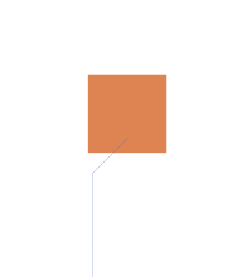
\includegraphics[scale=0.5]{images/turn-right-rimea1.png}
    \caption{Slight turn right in RiMEA scenario 1 run in Vadere with OSM \cite{osm, bridging-the-gap, dynamic-stride-length}.
    The orange square is the target and the blue line is the pedestrian's trajectory.}
    \label{fig:rimea1-turn-right}
\end{figure}

\paragraph{RiMEA scenario 6}
This scenario consists of 20 pedestrians moving around a left corner to reach a target.\\
In this case the differences between the implementation of exercise 1 and the one in Vadere with OSM are the following:
\begin{itemize}
    \item In exercise 1, the 20 pedestrians are places at random positions in the beginning of the corridor.
    This causes the pedestrians to start from different distances from the target, in some sense it is like the simulation had already started.
    In Vadere instead, it is possible to create a source that originates pedestrians from the same place in the map, making the simulation more realistic.
    
    \item The trajectories taken by pedestrians (Figure \ref{fig:rimea6}) are much more realistic using OSM compared to the ones in the exercise 1.
    Furthermore, it is possible to visualize them in the "Post-Visualization" in the GUI, while in the cellular automaton you could only try to track pedestrians moving at simulation time, making visual analyses much more difficult.\\
    Anyway, it is possible to observe in Figure \ref{fig:rimea6} some weird behaviors in the final part of the trajectories.
    Some pedestrians that are on the outside try to go to the center of the corridor for no apparent reason, and some of them do the opposite.
    By closely and slowly observing the simulation, however, it is possible to notice that pedestrians leave the center of the corridor when others are near them, but often they try to return to the center as soon as possible while they could just go straight (and this is what probably would happen in a real situation).
    
    \item The overall time necessary to make all the pedestrians reach the target is roughly 29.3 seconds.
\end{itemize}

\begin{figure}[H]
    \centering
    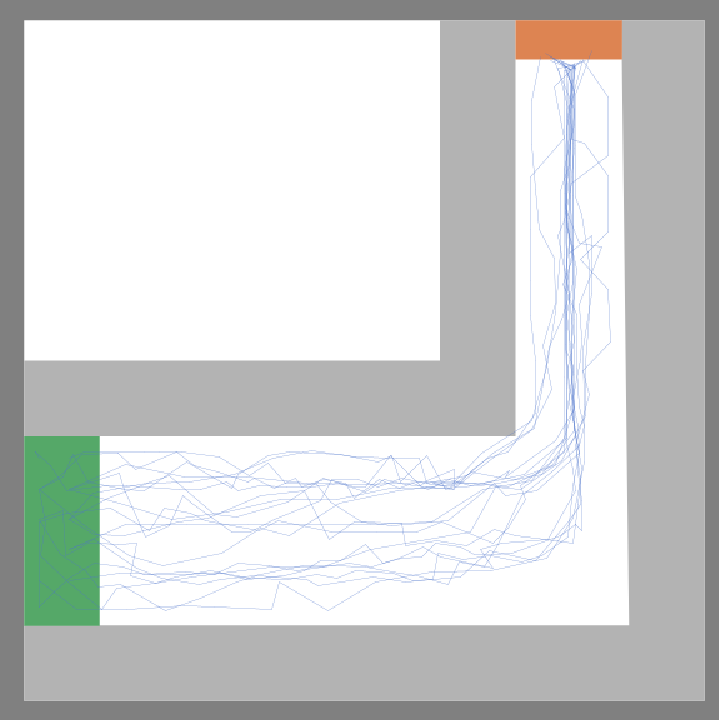
\includegraphics[scale=0.5]{images/rimea6-osm.png}
    \caption{RiMEA scenario 6 run in Vadere with OSM \cite{osm, bridging-the-gap, dynamic-stride-length}.}
    \label{fig:rimea6}
\end{figure}

\paragraph{Chicken test}
In this test there is one pedestrian in front of a target and they are separated by a U-shaped obstacle aimed to trap the pedestrian in case it goes straight towards the target.\\
In both the implementations of exercise 1 and Vadere with OSM the test is successfully passed, i.e. the pedestrian does not get trapped by the obstacle but it avoids it and reaches the target.
However the trajectories of the two implementations differ significantly:
\begin{itemize}
    \item Exercise 1: the trajectory is very squared, the pedestrian starts going in diagonal, perfectly at a 45° angle, then it coasts the border of the obstacle until it surpasses it and finally it goes 45° again to reach the target
    \footnote{Towards the end the pedestrian might actually move horizontally/vertically (and not diagonally) depending on the position of the target, but anyway it is matter of a single move in the last time step.}.
    In Figure \hyperref[fig:chicken-test]{\ref{fig:chicken-test}(a)} is is possible to see a reconstruction of the trajectory taken by the pedestrian in the exercise 1, using Dijkstra's algorithm.
    
    \item Vadere with OSM: as it is possible to observe in Figure \hyperref[fig:chicken-test]{\ref{fig:chicken-test}(b)}, the trajectory is more "rounded", but it looks less natural.
    A pedestrian, seeing such an obstacle, would go directly towards the external edge of it, instead here it goes towards the internal one, for then going right almost horizontally.
    The final third of the trajectory
    \footnote{After the vertical section, when the pedestrian surpasses the obstacle and starts going diagonally towards the target.}
    is a little more natural, even though it could be slightly more direct.\\
    The overall time to reach the target is roughly 7.9 seconds.
\end{itemize}

\begin{figure}[H]
    \centering
    \subfloat[a]{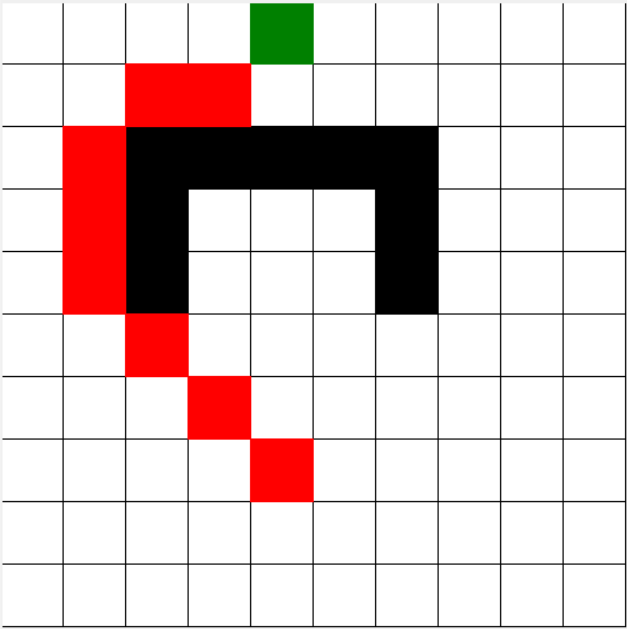
\includegraphics[width=0.4\textwidth]{images/chicken-test-ex1-dijkstra.png}}
    \hfill
    \subfloat[b]{
\includegraphics[width=0.4\textwidth]{images/chicken-test-osm.png}\label{fig:chicken-test-osm}}
    \caption{(a) The trajectory of the chicken test in exercise 1 using the Dijkstra's algorithm. (the trajectory has been recreated coloring in red the cells occupied by the pedestrian at each time step (from the bottom to the target (in green)). (b) the trajectory of the pedestrian running the OSM in Vadere.}
    \label{fig:chicken-test}
\end{figure}

% Ieas:
% \begin{itemize}
%     \item LEGGERE QUALCOSA SU OSM MODEL, così le differenze le vediamo esplicite e non "a occhio"
%     \item scaricare java jdk 11 per usare vadere
%     \item Differenze/similarità con il norstro es 1 in RIMEA scenario 1
%     \begin{itemize}
%         \item nel nostro il tempo era discreto, fixed time step. Tempo simulato = tempo reale, mentre qui il tempo simulato e quello reale possono differire (settando un ratio)
%         \item viene creato il file postvis.traj che salva posizione inizio e fine per ogni timestep
%         \item la velocità da noi è fissa (1.0m/s) mentre qui viene pescata pseudo-randomicamente per ogni pedestrian
%         \item OSM riesce nel chicken test
%     \end{itemize}
    
%     \item Differenze/similarità a livello di interfaccia
%     \begin{itemize}
%         \item possibilità di creazione di ostacoli poligonali non "quadrati"/ non solo con lati orizzontali e verticali
%         \item possibilità di creazione di sorgenti (multipli pedoni)
%         \item possibilità di cambiare da GUI il target absorbing o no
%         \item possibilità di cambiare da GUI un insieme di parametri sul pedone, velocità, particolare target di destinazione
%     \end{itemize}
% \end{itemize}

\end{task}


\begin{task}{2, Simulation of the scenario with a different model}
This task consists of running the 3 scenarios of task1 (RiMEA scenario 1, RiMEA scenario 2 and the chicken test) with the \textit{Social Force Model} (SFM) \cite{sfm1, sfm2} and the \textit{Gradient Navigation Model} (GNM) \cite{gnm, bridging-the-gap}.

\paragraph{Social Force Model (SFM)}
\begin{itemize}
    \item \textbf{RiMEA scenario 1:} in this simple test, the trajectory stays straight forward towards the target
    
    \item \textbf{RiMEA scenario 6:} in this case, the behavior exhibited using SFM is more natural than the one of OSM.
    All pedestrians tend to follow the optimal/shortest trajectory and they tend to be less repulsed by others.
    Furthermore, with SFM the paths are more smooth, while with OSM there are some hard angles and squared-like stretches.\\
    In Figure \hyperref[fig:rimea6-osm-sfm-gnm]{\ref{fig:rimea6-osm-sfm-gnm}(a)} and \hyperref[fig:rimea6-osm-sfm-gnm]{\ref{fig:rimea6-osm-sfm-gnm}(b)} it is possible to see the different trajectories between OSM and SFM.
    The ones of SFM look more natural especially in a running/panic/evacuation situation.\\
    Another thing noticeable observing the simulation, more then the trajectories, is that the crowd movement is more fluid in SFM because in OSM some pedestrian tend to give way to others in an excessive manner, stopping when it is not actually very necessary.\\
    The overall time necessary to make all the pedestrians reach the target is 25.2 seconds
    \footnote{It is worth noticing that, towards the end, only one single pedestrian, slower than the others, remains alone and makes the overall time increase significantly.}
    (with OSM it was 29.3 seconds).
    
    \item \textbf{Chicken test:} the test is of course passed also with SFM.
    Comparing to OSM, the trajectory is again a bit more direct, but anyway very similar.
    It is possible to compare the 2 trajectories visually in Figure \hyperref[fig:chicken-osm-sfm-gnm]{\ref{fig:chicken-osm-sfm-gnm}(a)} and \hyperref[fig:chicken-osm-sfm-gnm]{\ref{fig:chicken-osm-sfm-gnm}(b)}.\\
    The overall time to reach the target is 8.3 seconds (roughly 4 tenths of a second slower than OSM).
\end{itemize}

\paragraph{Gradient Navigation Model (GNM):}
\begin{itemize}
    \item \textbf{RiMEA scenario 1:} also using this model, the trajectory stays straight towards the target, as can be expected, given the simplicity of the scenario.
    
    \item \textbf{RiMEA scenario 6:} all the pedestrian really try to walk along the shortest path to the target (in Figure \hyperref[fig:rimea6-osm-sfm-gnm]{\ref{fig:rimea6-osm-sfm-gnm}(c)} it is possible to observe this line marked more heavily that runs next to the wall).
    This has the effect of "packing" the pedestrian together and this causes some slowdowns, especially for the pedestrian on the inside/tight line, who get their way continuously cut by the others that were on the outside.\\
    Overall the movements look still more natural than the ones obtained with OSM, but less so compared to the ones coming from an execution of the same scenario with SFM, in fact some slowdowns would be avoidable if some pedestrian would use the available space on the outside of the trajectory.\\
    The overall time necessary to make all the pedestrians reach the target is 27.6 seconds, making this model slower than SFM but quicker than OSM in the RiMEA scenario 6.
    
    \item \textbf{Chicken test:} the GNM takes a very directed trajectory to the target, it looks close to the shortest path that Dijkstra's algorithm could find.
    It is possible to observe this by comparing Figure \hyperref[fig:chicken-osm-sfm-gnm]{\ref{fig:chicken-osm-sfm-gnm}(c)} and Figure \hyperref[fig:chicken-test]{\ref{fig:chicken-test}(a)}.\\
    The overall time to reach the target is 8.0 seconds (OSM: 7.9s, SFM: 8.3s).
\end{itemize}

\begin{figure}[H]
    \centering
    \subfloat[a]{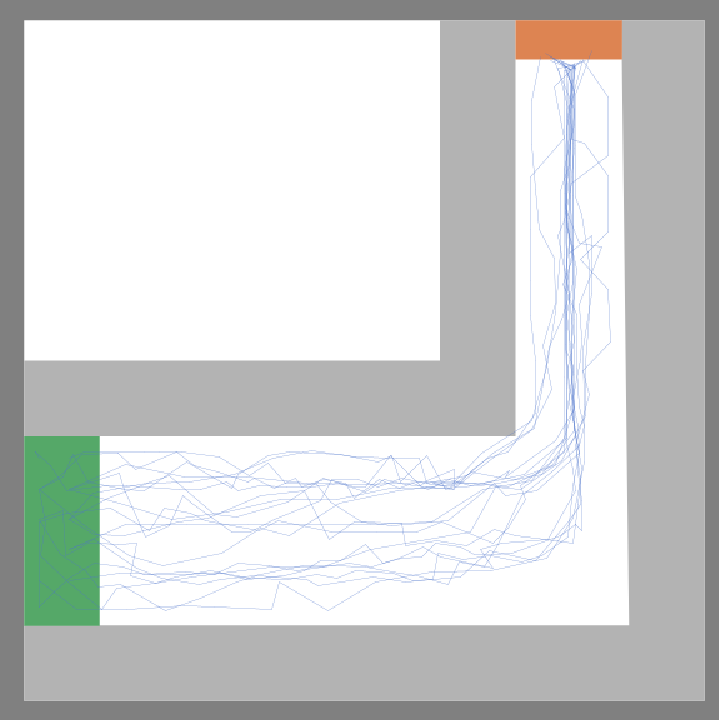
\includegraphics[width=0.3\textwidth]{images/rimea6-osm.png}}
    \hfill
    \subfloat[b]{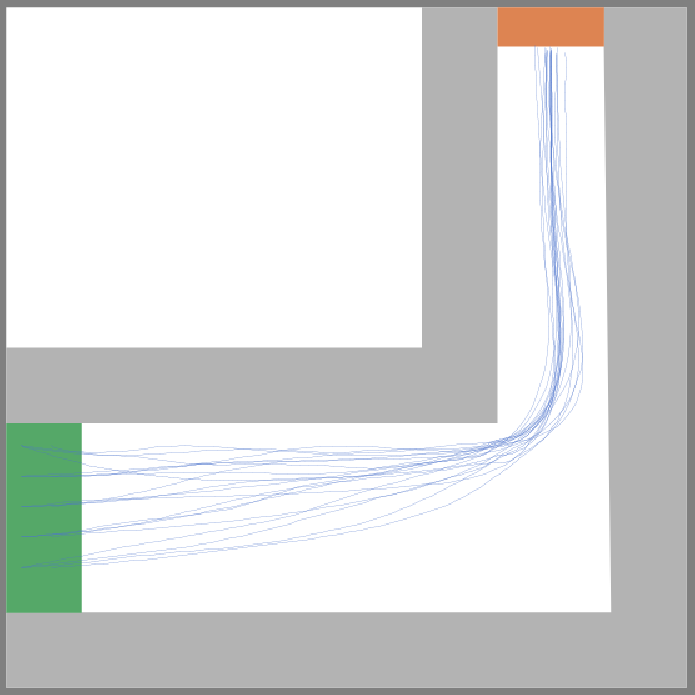
\includegraphics[width=0.3\textwidth]{images/rimea6-sfm.png}\label{fig:chicken-test-osm}}
    \hfill
    \subfloat[c]{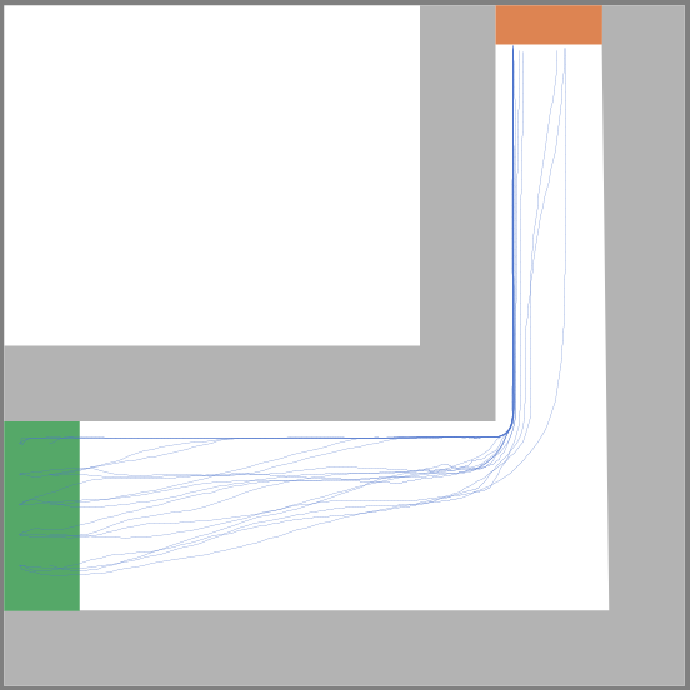
\includegraphics[width=0.3\textwidth]{images/rimea6-gnm.png}}
    \caption{The trajectories of the RiMEA scenario 6 run with OSM (a), with SFM (b) and with GNM (c).}
    \label{fig:rimea6-osm-sfm-gnm}
\end{figure}

\begin{figure}[H]
    \centering
    \subfloat[a]{
\includegraphics[width=0.3\textwidth]{images/chicken-test-osm.png}}
    \hfill
    \subfloat[b]{
\includegraphics[width=0.3\textwidth]{images/chicken-test-sfm.png}}
    \hfill
    \subfloat[c]{
\includegraphics[width=0.3\textwidth]{images/chicken-test-gnm.png}}
    \caption{The trajectory of the chicken test with OSM (a), with SFM (b) and with GNM (c).}
    \label{fig:chicken-osm-sfm-gnm}
\end{figure}
\end{task}


\begin{task}{3, Using the console interface from Vadere}
\paragraph{Running Vadere from console}
By running Vadere from console, instead of GUI, there are, as expected, no differences in the output files.
This check has been performed using the \texttt{diff} command of the Linux bash comparing file by file the outputs of two different runs of the same scenario, one with GUI and the other with console.

\paragraph{Adding pedestrians programmatically}
In order to be able to insert pedestrians programmatically, the script \texttt{add\_pedestrian.py} has been created.
It is a Python script that contains 3 functions, the main one being \texttt{add\_pedestrian}.\\
This function performs the following steps
\footnote{Only the main ones are reported in this report for a better clarity}:
\begin{itemize}
    \item \textbf{Get the scenario to modify:}
    the function takes as parameter either the path to the scenario file or the scenario itself in the form of a dictionary
    \footnote{In this case it means that a scenario file has already been read with json and the result of \texttt{json.load()} itself (i.e. a dictionary) is passed to the function.}.
    If the path is passed, the scenario is read with the help of \texttt{json.load()}.
    
    \item \textbf{Get the target id for the new pedestrian:}
    if the target id is not explicitly passed to the function, check if there is only one single target in the scenario and in that case set its id as the pedestrian's target id
    \footnote{This is an implementation choice, it would have been possible not to set the target id automatically in any case, but it was preferred to do it since most of the times each pedestrian has a target id, otherwise it wouldn't move.},
    otherwise leave this field blank (the pedestrian won't move in this case
    \footnote{If this is not the intended behavior, then the target ids must be passed explicitly.}).
    
    \item \textbf{Create the pedestrian:}
    it is simply a dictionary with the same structure (nested lists and dictionaries) present in the JSON file of the scenario under the key \texttt{dynamicElements}
    \footnote{In the scenario's JSON file, under the key \texttt{dynamicElements} it is the list of the pedestrians (the ones that are not originated from a source, to be precise).
    The pedestrian dictionary created in the function \texttt{add\_pedestrian} has the same structure of each of the elements in that list.}.
    Therefore, its structure and its keys are fixed and they have to mimic what found in the JSON file in order to be compatible, while the values associated to each key are passed to \texttt{add\_pedestrian} as parameters
    \footnote{Some values that were not in the interest of the tasks of this exercise are actually hard-coded and not passed as parameters.}.
    
    \item \textbf{Add the new pedestrian to the pedestrians list:}
    \begin{itemize}
        \item The list is obtained with: \texttt{scenario['scenario']['topography']['dynamicElements']}
        
        \item Add the new pedestrian (namely \texttt{ped}):\\ \texttt{scenario['scenario']['topography']['dynamicElements'].append(ped)}
    \end{itemize}
    
    \item \textbf{Save the output scenario:}
    with the help of \texttt{json.dump()}.
    This updated scenario file now contains the new pedestrian and can be loaded into Vadere.
\end{itemize}

\paragraph{Add pedestrian to RiMEA scenario 6}
At this point, it is possible to add a pedestrian in the desired position of the RiMEA scenario 6 simply by calling \texttt{add\_pedestrian} (described in previous paragraph).
An example of a call to this function is shown in Figure \hyperref[fig:callfunc-scen3]{\ref{fig:callfunc-scen3}(a)}, while the initial scenario for this task is displayed in Figure \hyperref[fig:callfunc-scen3]{\ref{fig:callfunc-scen3}(b)}.\\
The newly added pedestrian, starting from a location nearer to the target, reaches the destination first in 5.4 seconds, while the second fastest takes 8.9 seconds.\\
This test, since the base scenario is the one used in task 1, has been run with OSM.

\begin{figure}[H]
    \centering
    \subfloat[a]{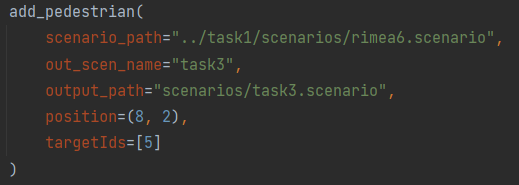
\includegraphics[width=0.4\textwidth]{images/example_call_add_predestrian.png}}
    \hfill
    \subfloat[b]{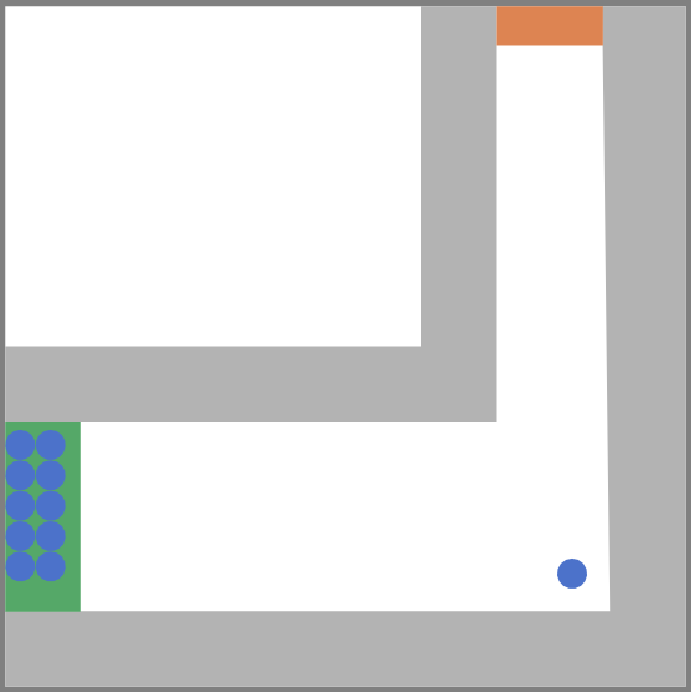
\includegraphics[width=0.4\textwidth]{images/scenario-task3.png}}
    \caption{(a) An example of a call to the function \texttt{add\_pedestrian}.
    (b) The initial scenario for this task.
    The isolated pedestrian has been added programmatically by a call like the one in (a).}
    \label{fig:callfunc-scen3}
\end{figure}
\end{task}


\begin{task}{4, Integrating a new model}
To integrate the proposed \texttt{SIR model} in Vadere the Moodle files have been positioned in the correct folders, as pointed out in the files first row of code. After re-building the software (using \textbf{IntelliJ 2021.2.3 (Community Edition)} and \textbf{Java JDK 11.0.13}) one can execute the modified Vadere software by executing the \texttt{VadereApplication} class. This original implemented model lacks some features and optimalities: it is composed only by \textit{infected} and \textit{susceptible} pedestrians, as well as not being properly colored nor properly initialized.

\textbf{\hyperref[fig:class-diagram]{Figure \ref{fig:class-diagram}}} gives an overview of the SIR model implementation in Vadere. Going more into detail:
\begin{itemize}
    \item \textbf{AttributesSIRG:} class to set some general parameters regarding the infection behavior.
    \begin{itemize}
        \item \textit{infectionsAtStart:} how many pedestrians have to be already infected at the start of the simulation.
        \item \textit{infectionRate:} how probable it is for a susceptible pedestrian to become infected if he/she is in contact with an infected pedestrian.
        \item \textit{infectionMaxDistance:} range in which a susceptible pedestrian gets the risk of being infected if another infected pedestrian is in that range.
    \end{itemize}
    \item \textbf{SIRGroup:} class to maintain an active counting and membership for different pedestrian groups. Each group, \textit{Infected, Susceptible and Recovered} in the proposed case, will keep a list of members.
    \begin{itemize}
        \item \textit{id:} to uniquely identify a pedestrian group.
        \item \textit{members:} list containing the pedestrians in the group. \texttt{addMember} and \texttt{removeMember} are responsible for the update of the list.
    \end{itemize}
    \item \textbf{SIRType:} \texttt{enum} \cite{enum} to conveniently store the possible pedestrian states.
    \item \textbf{SIRGroupModel:} main class, responsible for keeping the pedestrians divided in groups, updating them by actually performing infections (and later on possible recoveries).
    \begin{itemize}
        \item \textit{groupsById:} a \texttt{LinkedHashMap} to store the various present groups, identified by their id.
        \item \textit{attributesSIRG:} instance containing the aforementioned simulation parameters.
        \item \textit{totalInfected:} a counter to keep track of the overall number of currently infected.
        \item \texttt{getFreeGroupId:} creates groups for storing the infected and susceptible pedestrians, fulfilling also the \textit{attributesSIRG} initial constraints.
        \item \texttt{initializeGroupsOfInitialPedestrians:} assigns pedestrians in the scenario to groups at the beginning.
        \item \texttt{assignToGroup:} subroutine to assing a particular pedestrian to a group.
        \item \texttt{elementAdded:} wrapper of \texttt{assignToGroup}.
        \item \texttt{elementRemoved:} removes a pedestrian from a group.
        \item \texttt{update:} method which implements the model core. The method goes through every pedestrian, checks for infected nearer than maximal infective range. For every infected pedestrian found in the range a probability coin is tossed and if the pedestrian is unlucky then he/she becomes infected.
    \end{itemize}
    \item \textbf{FootStepGroupIDProcessor:} output processor to maintain the infection status in the resulting file, useful for later analysis and plotting. For a correct processing it is fundamental to assert this processor as the desired output processor, otherwise no infection status information will reach the post simulation.
    \begin{itemize}
        \item \texttt{doUpdate:} at each time step writes a new output row composed of the current time step, the pedestrian id and its group id.
    \end{itemize}
\end{itemize}

\begin{figure}[H]
    \centering
    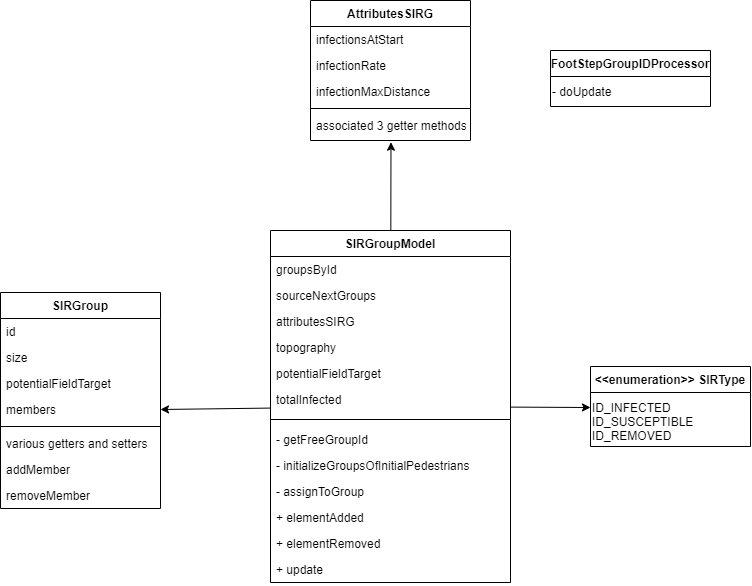
\includegraphics[scale=0.5]{images/SIRClassDiagram.drawio.png}
    \caption{slim version for the SIR model UML Class Diagram}
    \label{fig:class-diagram}
\end{figure}

After successfully integrating the SIR model into Vadere, some changes are needed for a fully working (and more efficient) implementation of such model. Namely the need for initial group assignment to pedestrians, the need for a correct coloring for better visualization and finally the need for a more efficient search for neighboring pedestrians during the \texttt{update}.
\begin{itemize}
    \item \textit{Initial group assignment:} without the initial assignment the future simulation updates call are useless and the simulation would not be respecting the constraints imposed by \textit{attributesSIRG}. In \textbf{\hyperref[fig:init-snippet]{Figure \ref{fig:init-snippet}}} it is possible to see the implementation inside a light blue box. A for loop iterates over all the pedestrians, calling indirectly the \texttt{getFreeGroupId} function for group assignment.
    \begin{figure}[H]
    \centering
    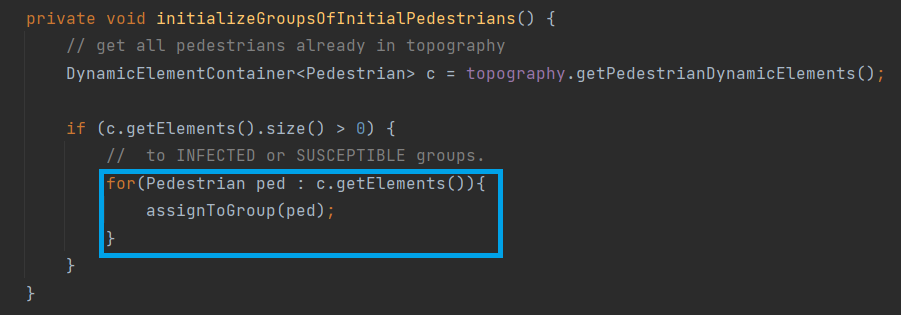
\includegraphics[scale=0.7]{images/simulation_initiation_snippet.png}
    \caption{initial group assignment snippet}
    \label{fig:init-snippet}
\end{figure}

    \item \textit{Correct coloring visualization:} the SIR groups are not visualized correctly in the initial setup, even after correct initial group assignment. A good and immediate visualization is absolutely fundamental when analysing behaviours, even though this coloring is not an issue neither for the output processor nor for the visualization scripts. To solve the problem a couple of lines have been added to \texttt{VadereGui/src/org/vadere/gui/components/model/SimulationModel.java}. More precisely, looking at \textbf{\hyperref[fig:color-snippet]{Figure \ref{fig:color-snippet}}}, the changes consist in adding the basic colors for the three different groups (orange box), changing the default simulator coloring agent (green box) and finally adding the mapping between group id and group coloring (red box). It is important to remark that this solution solves the problem regarding the simulation only, leaving the post visualization groups all identical in color as proposed in \textbf{\hyperref[fig:group-coloring-before-after]{Figure \ref{fig:group-coloring-before-after}}}.
\begin{figure}[H]
    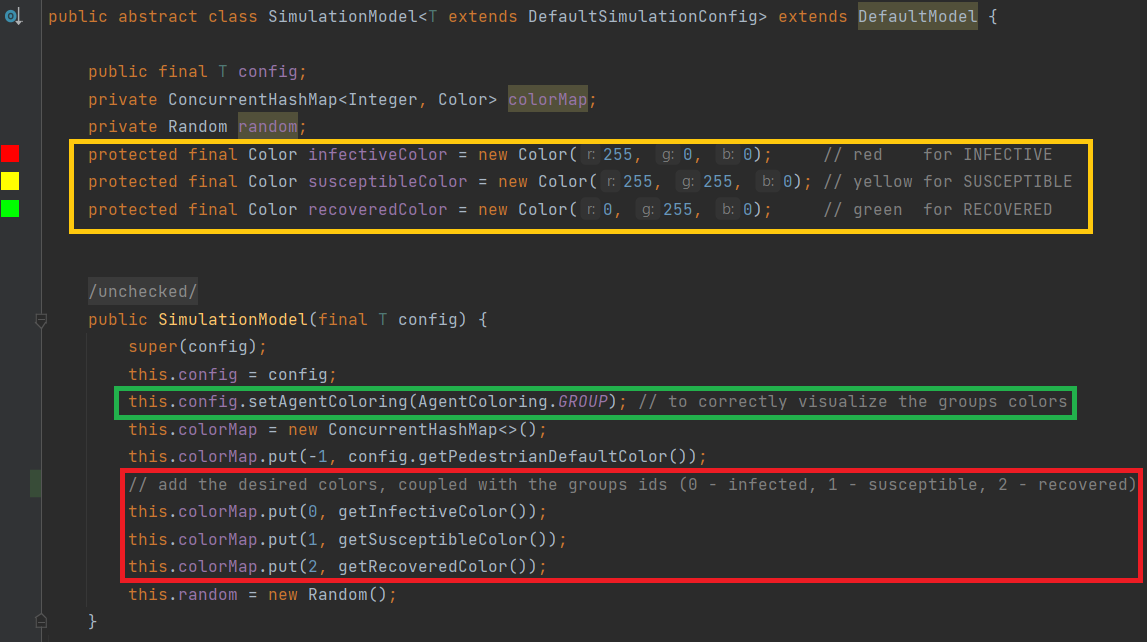
\includegraphics[scale=0.7]{images/simulation_coloring_snippet.png}
    \caption{simulation color correction snippet}
    \label{fig:color-snippet}
\end{figure}

\begin{figure}[!h]
  \centering
  \subfloat{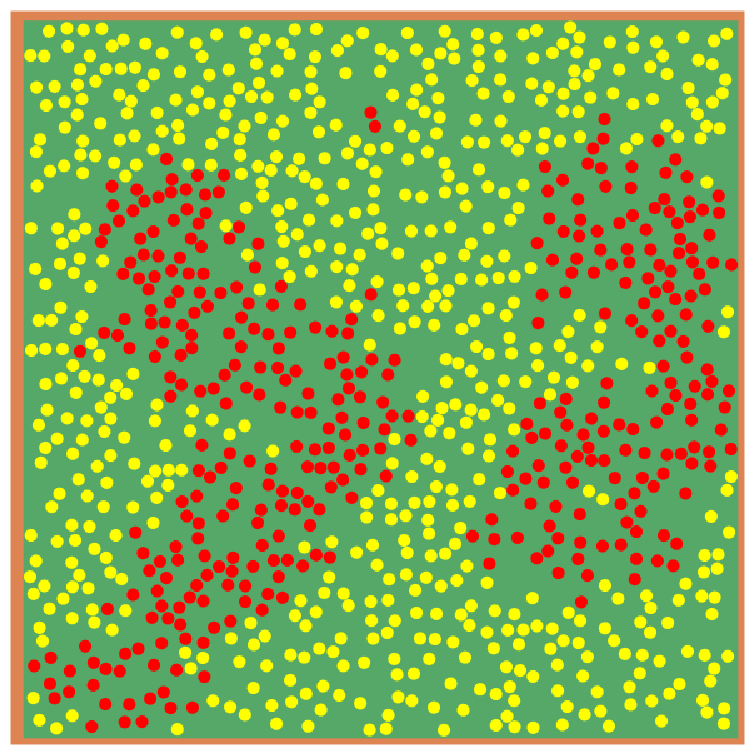
\includegraphics[width=0.3\textwidth]{images/during_sim.png}\label{fig:during-sim}}
  \hspace{2cm}
  \subfloat{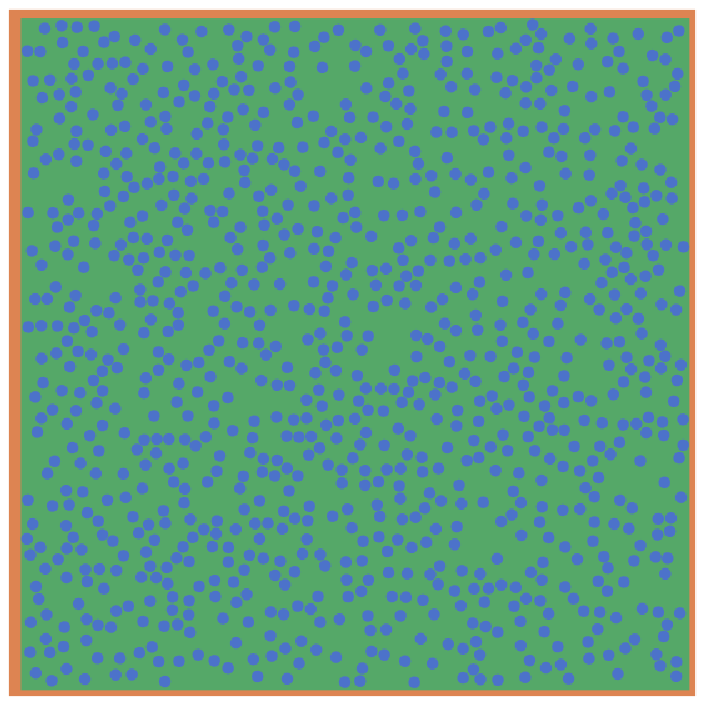
\includegraphics[width=0.3\textwidth]{images/after_sim.png}\label{fig:after-sim}}
\caption{Group coloring during and after the simulation}
\label{fig:group-coloring-before-after}
\end{figure}
    
\item \textit{Efficient search for neighboring pedestrians during the \texttt{update}:} originally the function was not efficient. For each pedestrian every other pedestrian would have been taken into consideration as plausible infective agent. In reality only those pedestrians who are both infectious and close enough to the current pedestrian are plausible for infection. This is anyway not the only inefficiency: all pedestrians are in fact checked for a change of state even if at the current state of the model only susceptible pedestrians are capable of changing state. Therefore it would be a good idea to act only on susceptible pedestrians and no others.\\ Both these situations have been solved as can be appreciated looking at the white box in \textbf{\hyperref[fig:optim-snippet]{Figure \ref{fig:optim-snippet}}}. If the current pedestrian is infected than no need to check its neighbours. If he/she is not infected, than, by having information on the cell elements, the current pedestrian will now look for infectious pedestrians only at its surroundings in the max infective range. This is possible thanks to the use of the \texttt{LinkedCellsGrid} class, which effectively implements a grid augmenting the position of generic objects (the pedestrian in this case), for faster access. Particularly useful resulted to be the \texttt{getObjects} method inside of the class, a method which exploits the constructed grid to get all the required neighbours of a given pedestrian. The method only needs the pedestrian position as \texttt{VPoint} object and the \texttt{radius} of search.


\begin{figure}[H]
    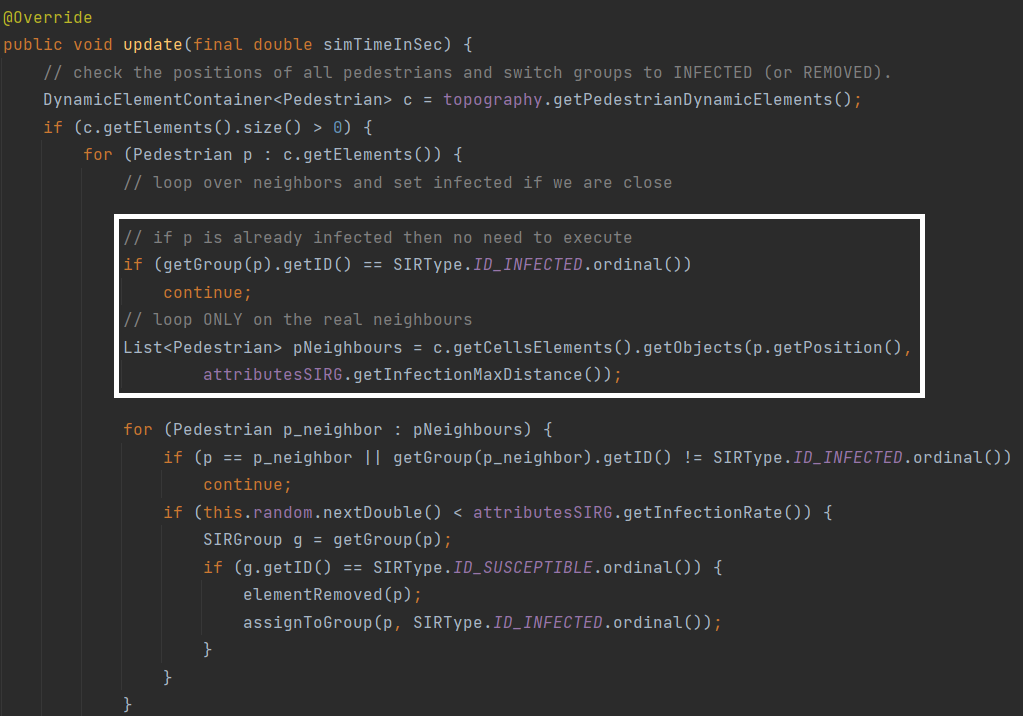
\includegraphics[scale=0.7]{images/simulation_optimization_snippet.png}
    \caption{simulation optimization snippet}
    \label{fig:optim-snippet}
\end{figure}
\end{itemize}

Once all the due fixes are in place it is possible to experiment with the modified Vadere software. In particular a couple of experiments have been carried out for this task:
\begin{itemize}
    \item a static scenario, where \textbf{1000} pedestrians are present and \textbf{10} are initially infected. The staticness is ensured by keeping the source on top of the target and making the target non-absorbing. The scenario is tested with different infection rate to state and appreciate the change in dynamic behaviour.
    \item a dynamic corridor scenario of \texttt{40mx20m} where a group of 100 susceptible pedestrians which are created overtime (the source attribute \texttt{useFreeSpaceOnly} is set to \texttt{true}) is moving from right to left and an automatically generated group of 100 infected pedestrians goes from left to right. The automatic generation is possible thanks to the code produced in \textbf{Task 3}, which is used as foundation for the script \texttt{create\_scenario\_task4.5\_2.py}, adding the 100 infected pedestrians on the left of the corridor. The objective is to grasp how many people get infected in the encounter between the two groups. 
\end{itemize}

Regarding the \textit{static scenario}, two experiments have been carried out:
\begin{itemize}
    \item \texttt{realTimeSimTimeRatio:0.1, simTimeStepLength:0.2} with the following infection parameters:\\ \texttt{infectionsAtStart:10, \textbf{infectionRate:0.01}, infectionMaxDistance:1.0}. An example of simulated behaviour can be appreciated in \textbf{\hyperref[fig:4.5.1]{Figure \ref{fig:4.5.1}}} where half of the population is infected in \textbf{47} seconds. 
    \item \texttt{realTimeSimTimeRatio:0.1, simTimeStepLength:0.2} with the following infection parameters:\\ \texttt{infectionsAtStart:10, \textbf{infectionRate:0.02}, infectionMaxDistance:1.0}. A similar behaviour happens to the one previously shown in \textbf{\hyperref[fig:4.5.1]{Figure \ref{fig:4.5.1}}}, with the difference standing obviously in the infection spreading faster. Half of the population is infected in fact in only \textbf{21} seconds, less than half of the previously reported time. 
\end{itemize}

\begin{figure}[H]
    \centering
    \subfloat[a]{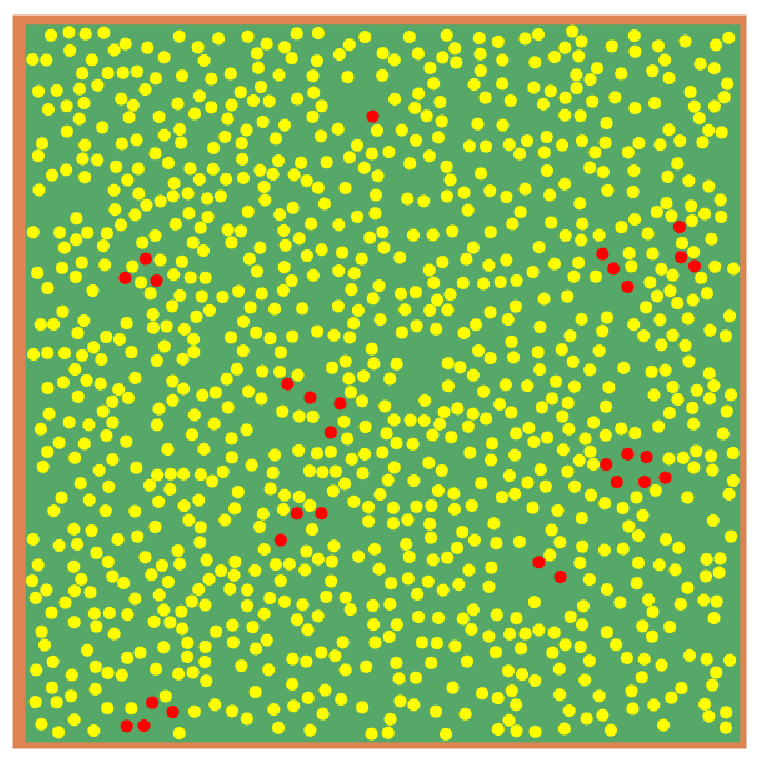
\includegraphics[width=0.3\textwidth]{images/4.5/4.5.1/init.png}\label{fig:4.5.1-1}}
    \hfill
    \subfloat[b]{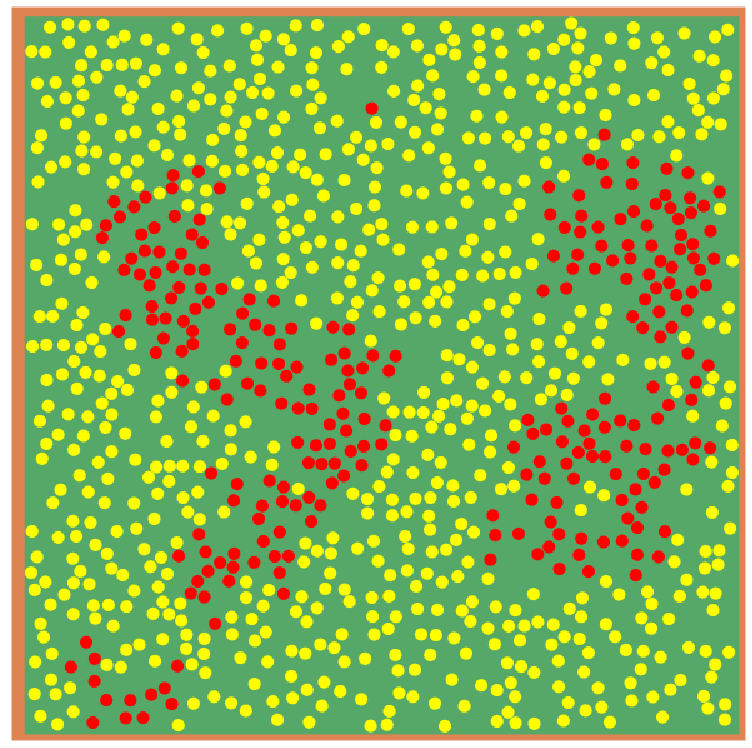
\includegraphics[width=0.3\textwidth]{images/4.5/4.5.1/mid.png}\label{fig:4.5.1-2}}
    \hfill
    \subfloat[c]{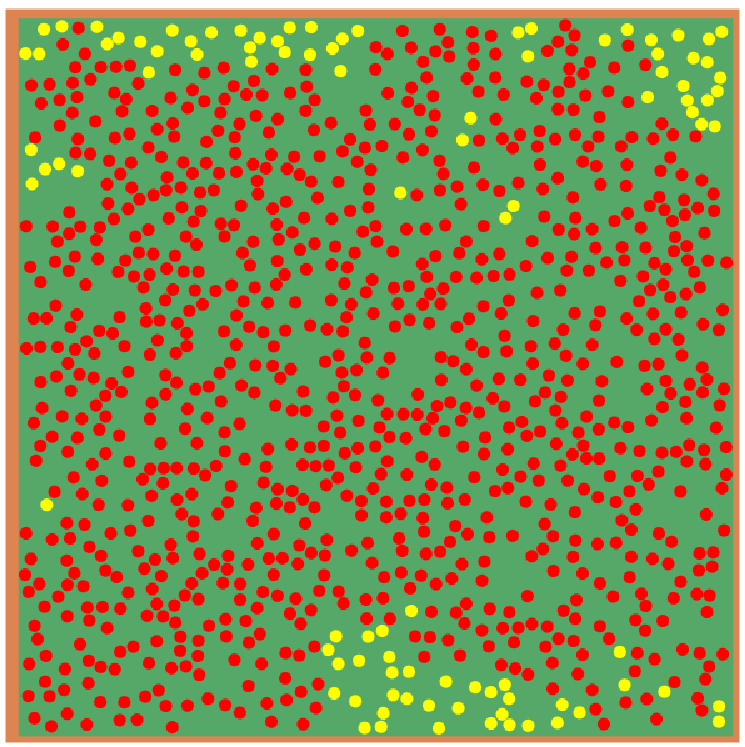
\includegraphics[width=0.3\textwidth]{images/4.5/4.5.1/near_end.png}\label{fig:4.5.1-3}}
    \caption{Simulation evolution from left to right.}
    \label{fig:4.5.1}
\end{figure}

Using the \textit{Dash/Plotly} visualization utility it is possible to better graphically describe the flow of infection, both for the single simulation and the multiple simulations (\textbf{\hyperref[fig:dash-4.5.1]{Figure \ref{fig:dash-4.5.1}}}). The graphic immediately shows how the higher infection rate delivers a much faster infection spreading, with the susceptible getting all infected in a visibly shorter time.

\begin{figure}[!h]
  \centering
  \subfloat{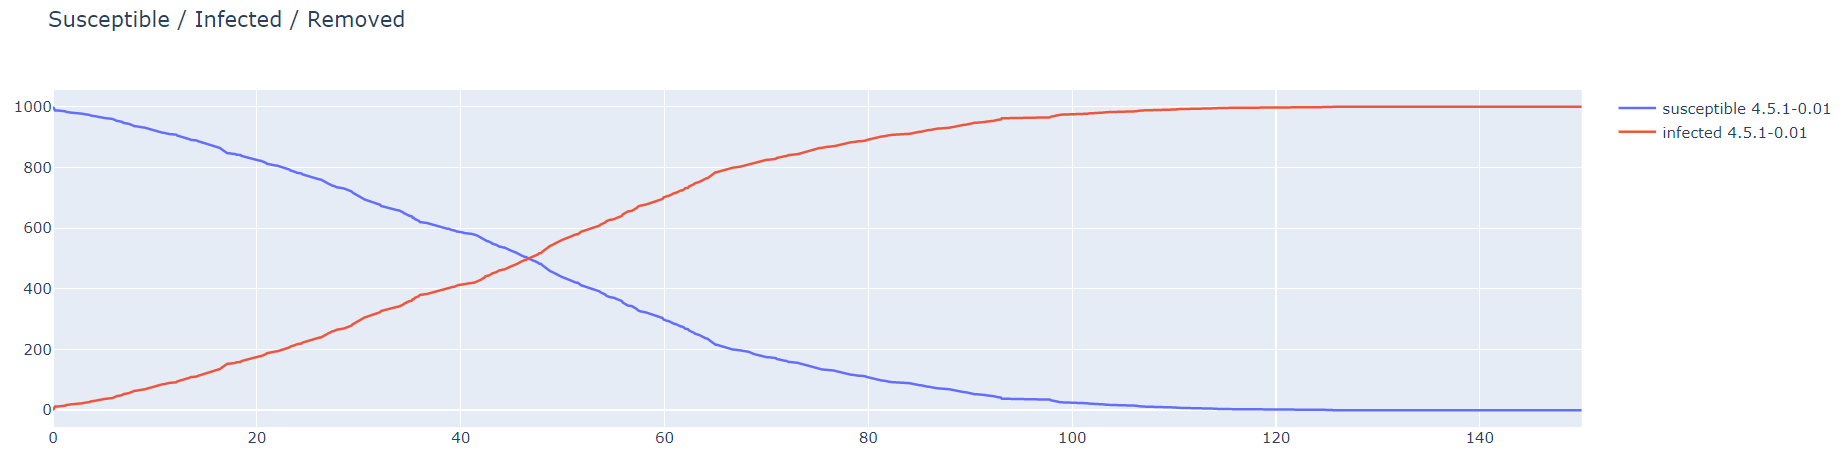
\includegraphics[width=1\textwidth]{images/4.5/4.5.1/0.01.png}\label{fig:single-dash-4.5.1}}
  \vspace{1cm}
  \subfloat{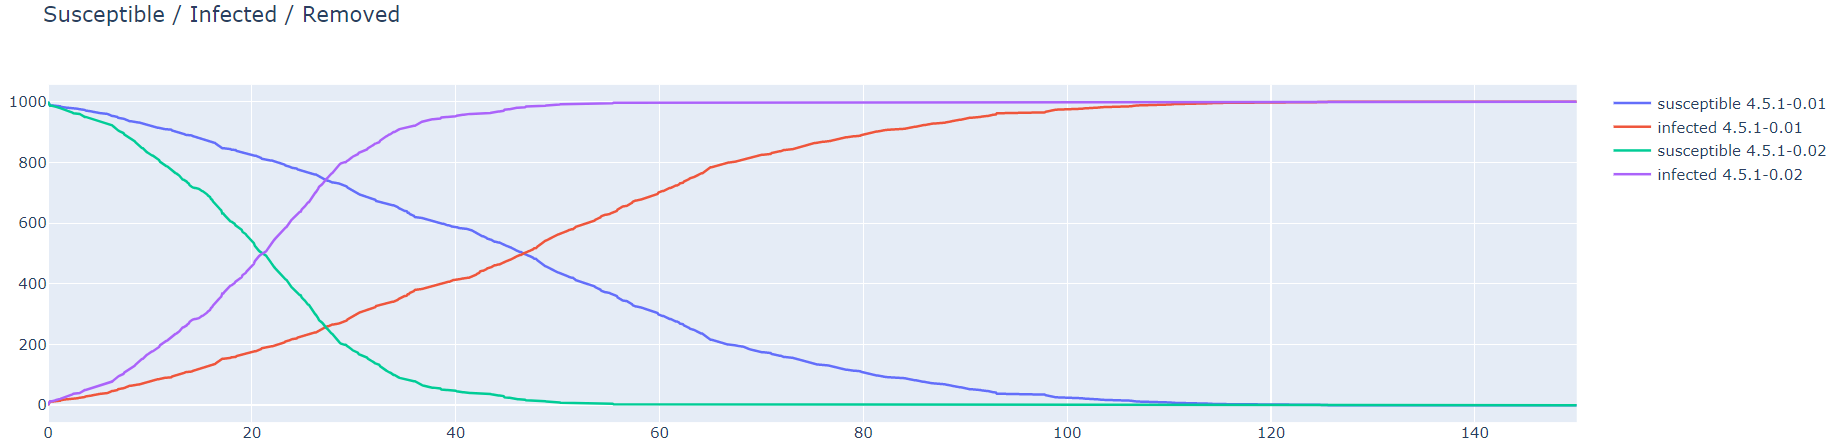
\includegraphics[width=1\textwidth]{images/4.5/4.5.1/0.02.png}\label{fig:multiple-dash-4.5.1}}
\caption{Single (above) and multiple (below) simulation - time on the x, pedestrians on the y}
\label{fig:dash-4.5.1}
\end{figure}

\pagebreak
Regarding the \textit{corridor scenario}, the two groups run into each other and interact in the middle of the scenario. Both a simple notebook (\texttt{analyze\_corridor\_counterflow\_infections.ipynb}) and the \textit{Dash/Plotly} (\textbf{\hyperref[fig:corridor-dash]{Figure \ref{fig:corridor-dash}}}) are able to identify that during the interaction \textbf{21} healthy pedestrians get infected. The scenario has the following parameters: \texttt{realTimeSimTimeRatio:1.0, simTimeStepLength:0.2, infectionsAtStart:0, infectionsRate:0.1, infectionsMaxDistance:1.0}.\\
\textbf{\hyperref[fig:4.5.2]{Figure \ref{fig:4.5.2}}} portrays an evolution of the simulated scenario, showing the interaction between the groups. The groups get slowed down during the interaction because of the higher density in the area, simulating well a real world scenario. In the \textit{Dash/Plotly} figure the interaction moment is easily identifiable, with the infection curve rising and then stabilizing again once the two groups get past each other.

\begin{figure}[H]
    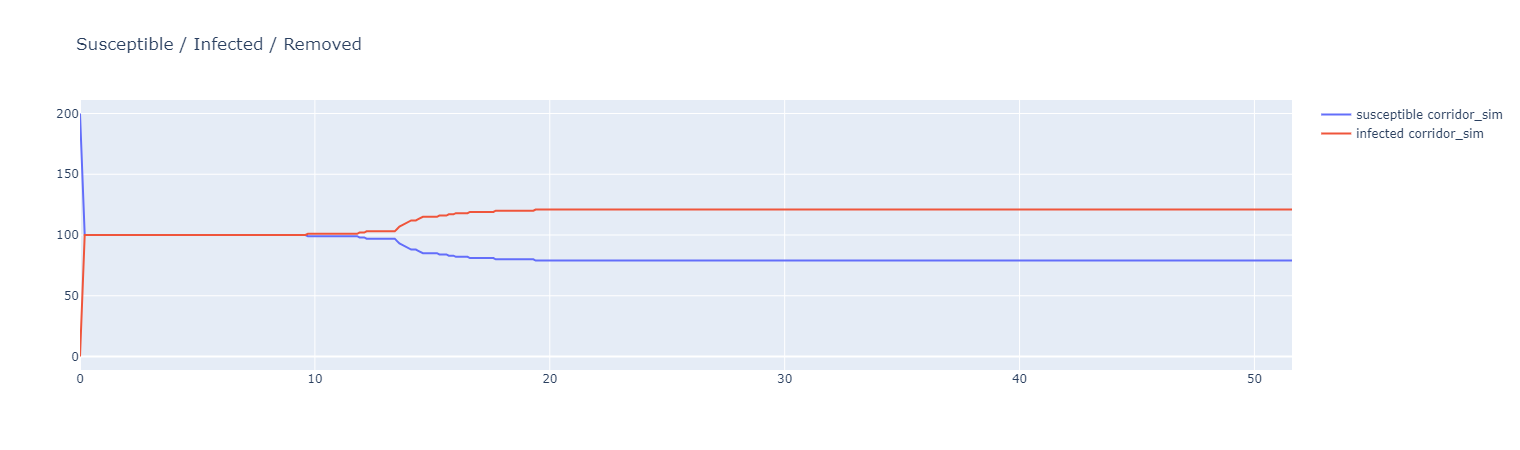
\includegraphics[scale=0.3]{images/4.5/4.5.2/corridor_dash.png}
    \caption{Dash visualization of corridor scenario}
    \label{fig:corridor-dash}
\end{figure}

\begin{figure}[H]
    \centering
    \subfloat[a]{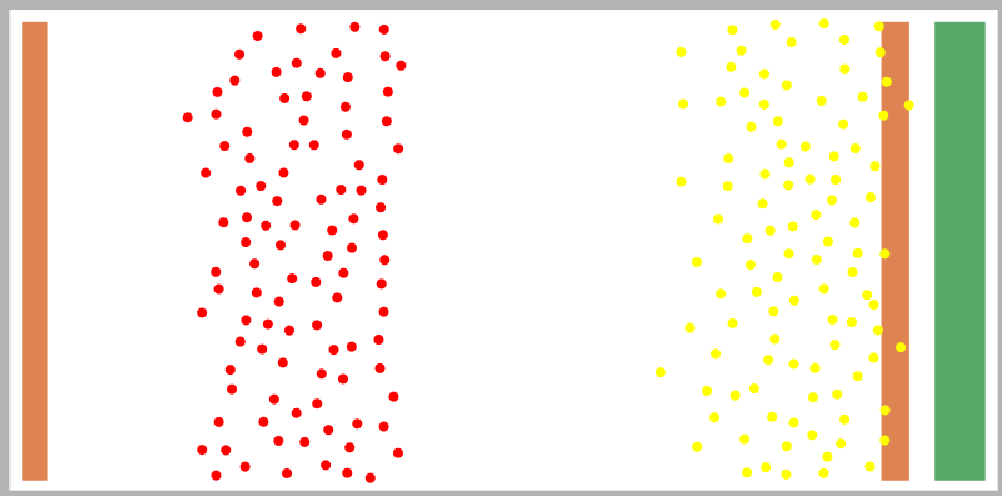
\includegraphics[width=0.6\textwidth]{images/4.5/4.5.2/mid_c.png}\label{fig:4.5.2-1}}
    \vfill
    \subfloat[b]{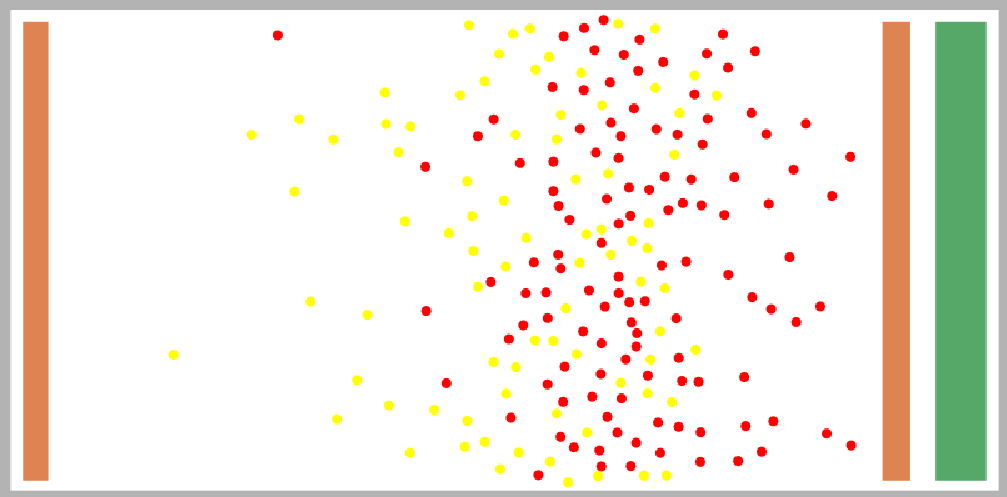
\includegraphics[width=0.6\textwidth]{images/4.5/4.5.2/after_c.png}\label{fig:4.5.2-2}}
    \vfill
    \subfloat[c]{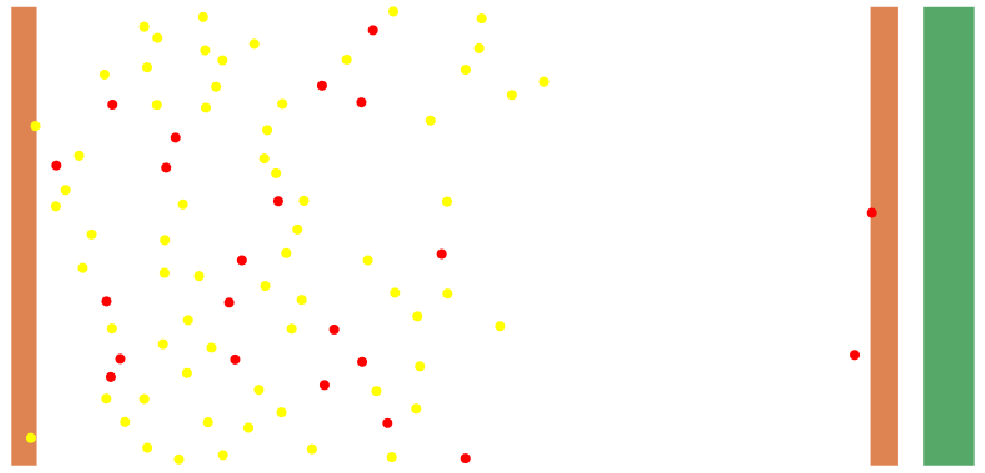
\includegraphics[width=0.6\textwidth]{images/4.5/4.5.2/end_c.png}\label{fig:4.5.2-3}}
    \caption{Simulation evolution from left to right.}
    \label{fig:4.5.2}
\end{figure}

Even though the simulation behaviour seems to be realistic, an unnatural mechanism is still present. If one were to change the \texttt{simTimeStepLength} parameter then a different result comes out of the \textit{corridor scenario}, as well as in any other scenario. The problem stands in the fact that the \texttt{SIRGroupModel} update function, responsible for new infections (and later on for new recovered pedestrians), is called at every simulation time step, making it so that the bigger the time step the littler the updates and the probability of new infections, and viceversa. A decoupling between the simulated step length and the \texttt{SIRGroupModel} update is possible and should therefore be present.\newline
A possibility for decoupling could be changing the \texttt{SIRGroupModel} update frequency such that it becomes independent from the simulated time step. Exploiting the simulated time step range (in Vadere it stands betwen 0.0 and 1.0 excluded), the proposed solution is to update the \texttt{SIRGroupModel} only \textbf{once per second}, keeping therefore a perhaps higher discretization but giving back nevertheless a detached update from the simulated time step granularity. It is relevant to notice that the \textit{once per second} is an a priori decision which can be modelled to be whatever frequency seems to best fit, the proposed solution is simply an example of which frequency could be chosen.\newline
The solution implementation is relatively simple: \texttt{SIRGroupModel} class is not changed at all, the code changes earlier on in the execution hierarchy. The \texttt{SIRGroupModel update} method is in fact called by the \texttt{Simulation} class via \texttt{updateLocomotion} method, which calls periodically (at every simulated time step) for an update of every model. The proposed solution makes the execution of an update of \texttt{SIRGroupModel} possible only if a second has passed from the last call, as can be appreciated in the purple box of the code snippet in \textbf{\hyperref[fig:decouple-snippet]{Figure \ref{fig:decouple-snippet}}}.\newline
The effect of this implementation is that no matter what are the \texttt{realTimeSimTimeRatio, simTimeStepLength} the simulated behaviour will be definitely more realistic and coherent with the passing time.

\begin{figure}[H]
\centering
    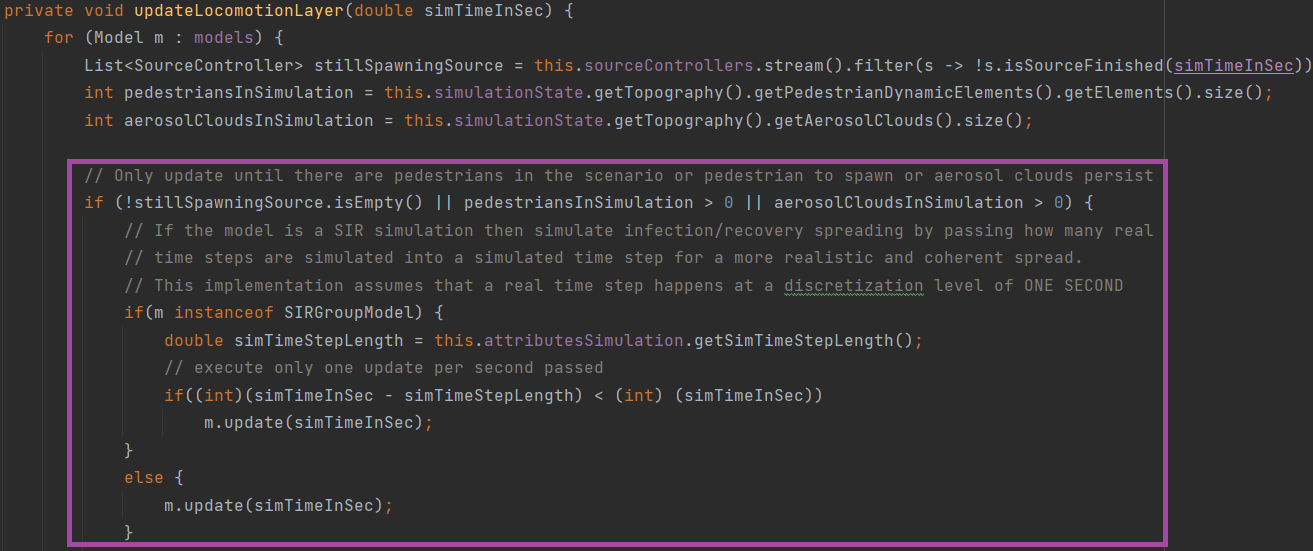
\includegraphics[scale=0.5]{images/4.6.png}
    \caption{decoupling of \texttt{SIRGroupModel} update}
    \label{fig:decouple-snippet}
\end{figure}

At the end of the task, it is interesting to discuss possible extensions that such a malleable model can be adapted to have. Regarding the addition of new states:
\begin{itemize}
    \item \textit{Dead:} with every probability not the most original idea but nevertheless important and realistic (nowadays more than ever!) in the proposed scenario. Infections can of course lead to death, creating a new pedestrian state where the pedestrian would become static (\textit{no target id}) and non-infective as well as non - infectable.
    \item \textit{Vaccinated:} once again an ever more realistic feature to represent realistically an infection scenario. It could be in fact plausible to sustain that after a certain period of time vaccines can become available against a certain pathology. Infected, susceptible and recovered could all become vaccinated with a certain rate of possibility. In the vaccinated state pedestrians have a much lowered infection rate, a higher recovery rate and also a much lower death rate, implying the previously proposed rate is already implemented.
    \item \textit{Immune:} someone is luckier than others, genetics plays an important role in having a different response to pathology exposure. This fact is absolutely present in the human nature, implying the utility of such a state. This state would be assigned at the start of the simulation, and only in that moment, with a certain rate. A pedestrian in the immune state cannot ever become susceptible, infected or recovered.
\end{itemize}
Another possible idea to make the simulation more realistic and dynamic could be the addition of \textit{aging/pedestrians having different ages to start with}. In reality we have in fact different ages, which makes us on average differently susceptible to illnesses. At an implementation point of view the pedestrian age could be chosen from a distribution and the age would act as a weight on the infection/recovery/death rate. Going more in depth, an aging mechanism could be added so that as time passes the pedestrians get older, therefore dynamically changing their infection/recovery/death rate.
\end{task}


\begin{task}{5, Analysis and visualization of results}
After having integrated the SIR model into Vadere in the previous task, now it has been expanded with new features related to a new state that a pedestrian can assume: \textbf{recovered}.\\
A pedestrian can switch to recovered only from infected, and once reached this state, it cannot change (i.e. it cannot be re-infected or become susceptible to infection).\\
To add this feature, different steps were necessary and the following modifications have been brought to the following classes/enums:
\begin{itemize}
    \item \texttt{SIRType}:
    the unused item \texttt{ID\_REMOVED} has been changed to \texttt{ID\_RECOVERED}.
    
    \item \texttt{AttributesSIRG}:
    the \texttt{recoveryRate} attribute has been added, which is the equivalent of \texttt{infectionRate} but for pedestrians' recoveries.
    
    \item \texttt{SimulationModel}:
    \begin{itemize}
        \item three attributes of type \texttt{Color} were added to represent the colors associated with different pedestrians' states: \texttt{infectiveColor} (red), \texttt{susceptibleColor} (yellow) and \texttt{recoveredColor} (green).
        
        \item in the constructor, the parameter that determines the color of the pedestrians has been changed from the target they are pointing to the group they belong to (susceptible, infected or recovered).
        Furthermore the desired colors for the different groups have been added to the attribute \texttt{colorMap}.
        The updated constructor is shown in Figure \ref{fig:simmodel-constructor}.
        
        \item the "getter" methods for the newly added attributes (\texttt{infectiveColor}, \texttt{susceptibleColor} and \texttt{recoveredColor}) were added.
    \end{itemize}
    
    \item \texttt{SIRVisualization} module:
    \begin{itemize}
        \item \texttt{app.py}:
        very few changes were necessary to this file, in fact we only changed the title of the plot adding the word "Recovered" in the function \texttt{update\_figure}.
        Within this function, \texttt{create\_folder\_data\_scatter} is called.
        It is a function contained in \texttt{SIRVisualization.utils.py} and this has indeed been modified.
        
        \item \texttt{utils.py}:
        \begin{itemize}
            \item function \texttt{file\_df\_to\_count\_df}:
            the attribute \texttt{ID\_RECOVERED} has been added and the function's body (showed in Figure \ref{fig:file_df_to_count_df}) has been changed in order to consider the recovered pedestrians.\\
            In particular these operations are performed:
            for every pedestrian, save a dataframe \cite{pandas-df} called \texttt{simtime\_group} containing the simulation time and the group id (susceptible/infected/recovered) at that time for the current pedestrian and save the current state as the group to which the pedestrian belongs at the beginning of the simulation (first time step).
            Then save another dataframe (\texttt{group\_counts}) containing the again simulation time and then 3 columns - one for each group - containing the number of pedestrians belonging to that group at that time.
            Finally, start iterating over the rows of the first dataframe (i.e. over the time steps) and:
            \begin{itemize}
                \item if the pedestrian passes from susceptible to infected, save the current state to infected and for all the next time steps increase the number of infected people and decrease the one of the susceptible people in \texttt{group\_counts}.
                
                \item if then it passes from infected to recovered, increase the number of recovered people for all the next time steps and decrease the one of infected people.
                Since the state cannot change from "recovered", exit the iteration over the time steps and go to the next pedestrian.
            \end{itemize}
        \end{itemize}
    \end{itemize}
\end{itemize}

\begin{figure}[H]
    \centering
    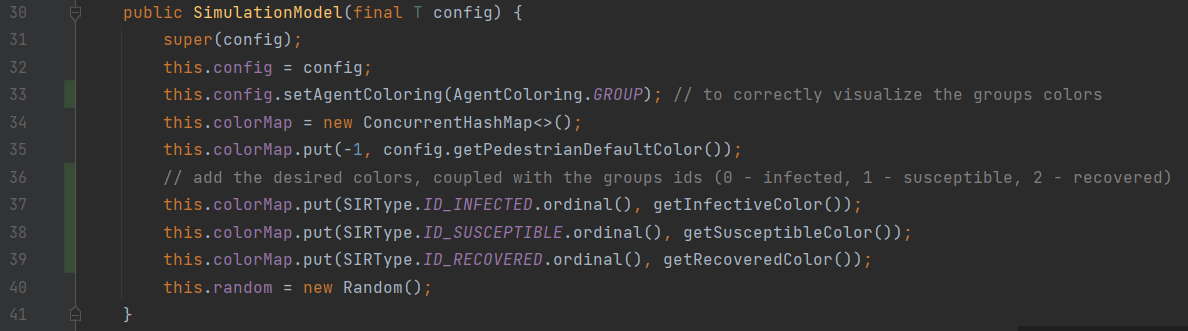
\includegraphics[scale=0.7]{images/SimulationModel-constructor.png}
    \caption{The updated constructor of \texttt{SimulationModel}.
    At line 33 the argument of \texttt{config.setAgentColoring} has been changed from \texttt{AgentColoring.TARGET} to \texttt{AgentColoring.GROUP}.
    Lines 37, 38 and 39 set the desired colors for the 3 states in the \texttt{colorMap}.}
    \label{fig:simmodel-constructor}
\end{figure}

\begin{figure}[H]
    \centering
    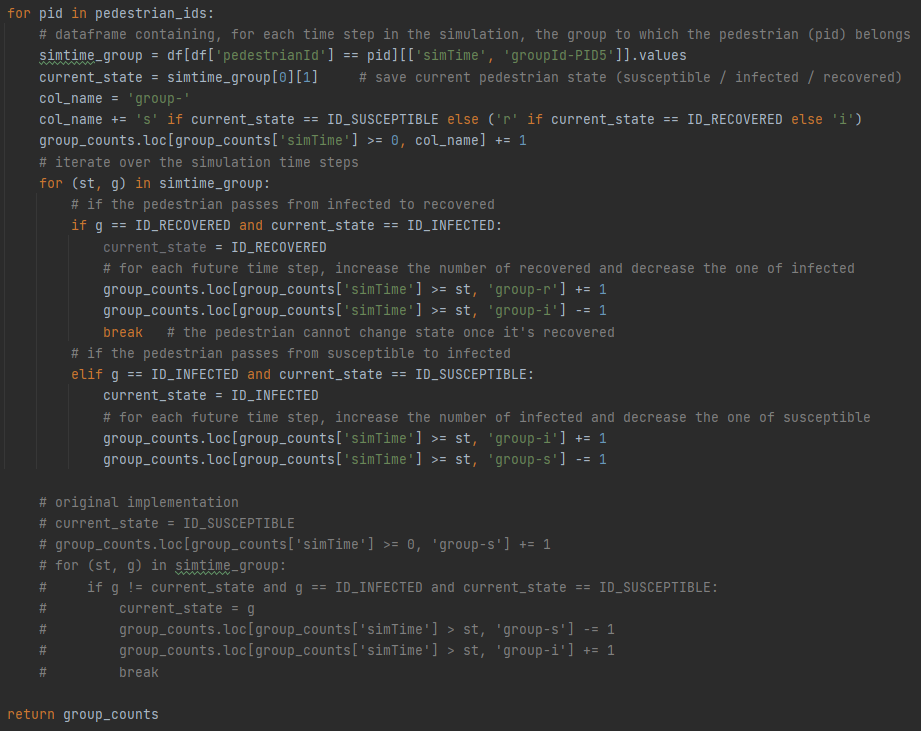
\includegraphics[scale=0.75]{images/file_df_to_count_df.png}
    \caption{The body of the function \texttt{file\_df\_to\_count\_df}.
    The commented lines show the code previous to the modifications introduced to take the recovered pedestrians into account.}
    \label{fig:file_df_to_count_df}
\end{figure}

To test the implementation of this new state ("recovered"), the same test presented for the previous task has been performed:
1000 pedestrians are placed on a grid, 990 susceptible and 10 infected.
They do not move but they can infect each other according to the SIR model with the addition of the "recovered" state.\\
This test has been run with different configurations for the infection rate and the recovery rate.
Some plots are available on \textbf{Figure \ref{fig:inf-rec-rates-plots}} and some screenshots of the execution of the scenarios are present in \textbf{Figure \ref{fig:inf-rec-rates-screenshots}}.
The different rates configurations are:
\begin{enumerate}
    \item Infection rate equal to recovery rate (actual value: 0.01):
    here the infection is well contrasted by the recoveries, in fact in spreads pretty slowly among pedestrian.
    The infection is finally blocked and by the end of the run the situation stabilizes having slightly less than 400 pedestrians that have not been infected.
    The final number of recovered is 600 ca., meaning that more than half of the population has been infected.
    
    \item Infection rate double than the recovery rate (actual values: 0.02 and 0.01):
    in \textbf{Figure \hyperref[fig:inf-rec-rate-plots]{\ref{fig:inf-rec-rates-plots}(b)}} it is possible to see how, by the end of the simulation, almost everyone had been infected, because the number of recovered people is near 1000 (i.e. the whole population).
    Recall that in order to be recovered, one must have been infected first.
    
    \item Infection rate half of the recovery rate (actual values: 0.01 and 0.02):
    in this third case, the infection starts spreading, but it gets controlled by the fast recovery rate of the pedestrians.
    By the end, only slightly more than 200 people (20\% of the population) got infected.
\end{enumerate}

\begin{figure}[H]
    \centering
    \subfloat[a]{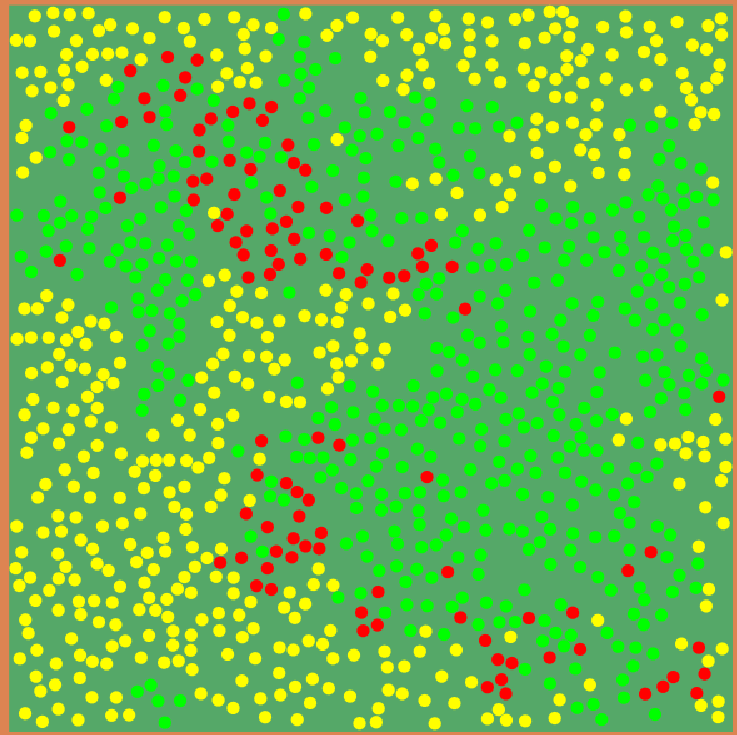
\includegraphics[width=0.4\textwidth]{images/inf01-rec01-screenshot.jpg}}
    \hfill
    \subfloat[b]{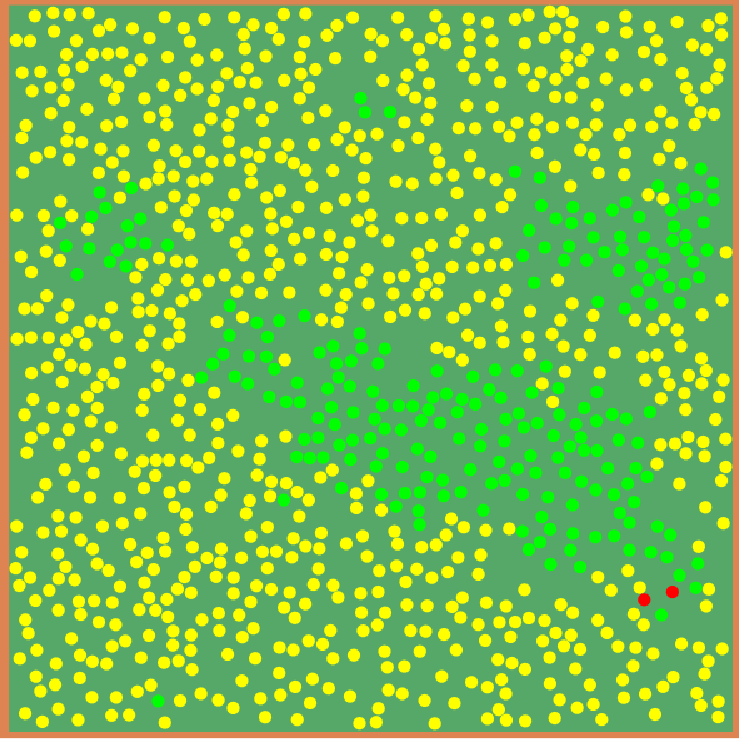
\includegraphics[width=0.4\textwidth]{images/inf01-rec02-screenshot.jpg}}
    \hfill
    \subfloat[c]{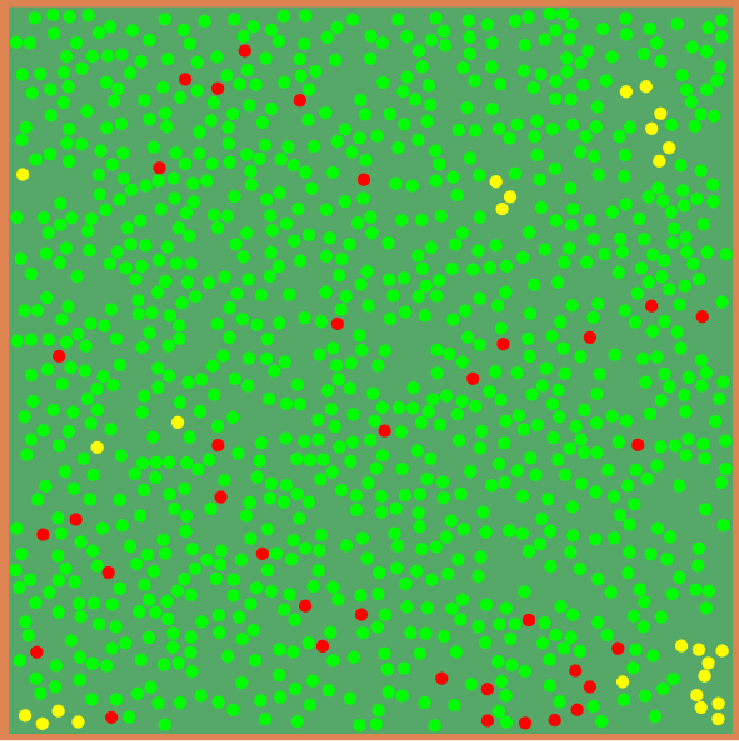
\includegraphics[width=0.4\textwidth]{images/inf02-rec01-screenshot.jpg}}
    \caption{Screenshots of the scenarios while run with different infection and recovery rates, namely:
    (a) infection rate = 0.1 and recovery rate = 0.1;
    (b) infection rate = 0.1 and recovery rate = 0.2;
    (c) infection rate = 0.2 and recovery rate = 0.1}
    \label{fig:inf-rec-rates-screenshots}
\end{figure}

\begin{figure}[H]
    \centering
    \subfloat[a]{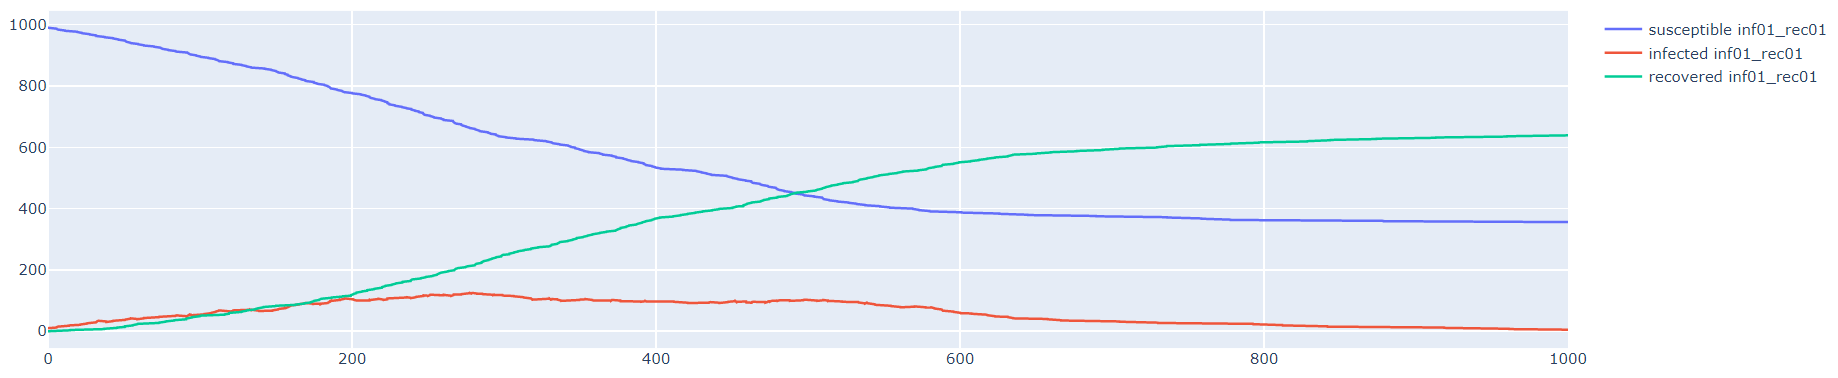
\includegraphics[width=0.9\textwidth]{images/inf01-rec01-plot.jpg}}
    \vfill
    \subfloat[b]{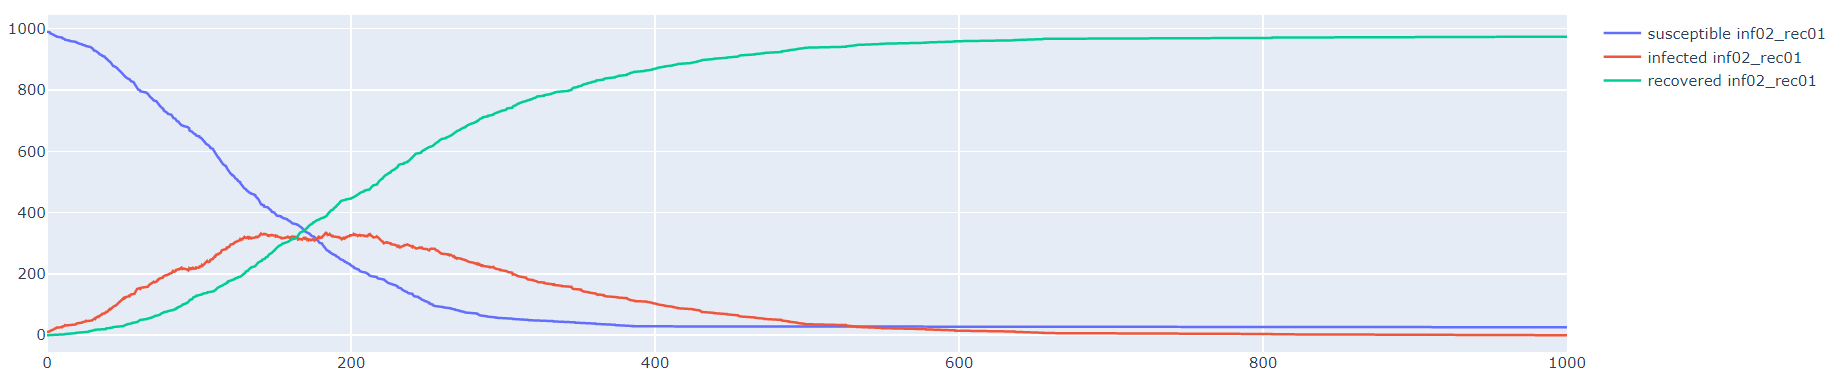
\includegraphics[width=0.9\textwidth]{images/inf02-rec01-plot.jpg}}
    \vfill
    \subfloat[c]{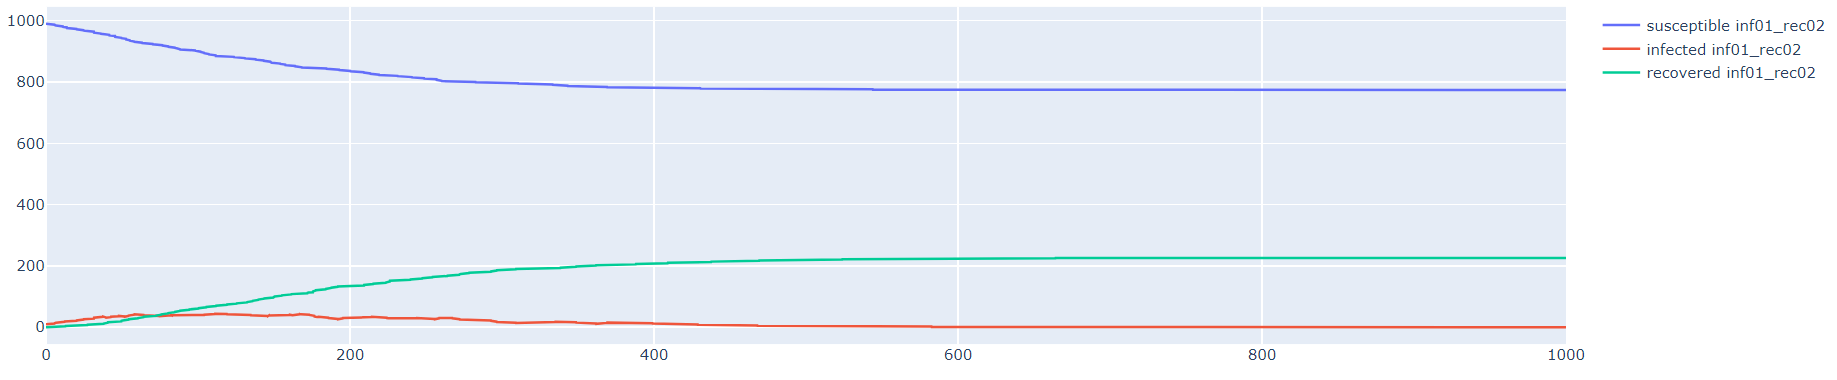
\includegraphics[width=0.9\textwidth]{images/inf01-rec02-plot.jpg}}
    \caption{Evolution of the number of susceptible, infected and recovered pedestrian with
    (a) infection rate = 0.1 and recovery rate = 0.1;
    (b) infection rate = 0.2 and recovery rate = 0.1;
    (c) infection rate = 0.1 and recovery rate = 0.2}
    \label{fig:inf-rec-rates-plots}
\end{figure}

Eventually one last test was carried on to verify how the model behaves in a real world scenario of infection: a supermarket. The supermarket is in fact a plausible site of disease spreading, where careful considerations should be made to avoid gatherings or a too reduced interpersonal space. The proposed supermarket scenario is the one proposed in \textbf{\hyperref[fig:intro-supermarket]{Figure \ref{fig:intro-supermarket}(a)}}.

\begin{figure}[H]
    \centering
    \subfloat[a]{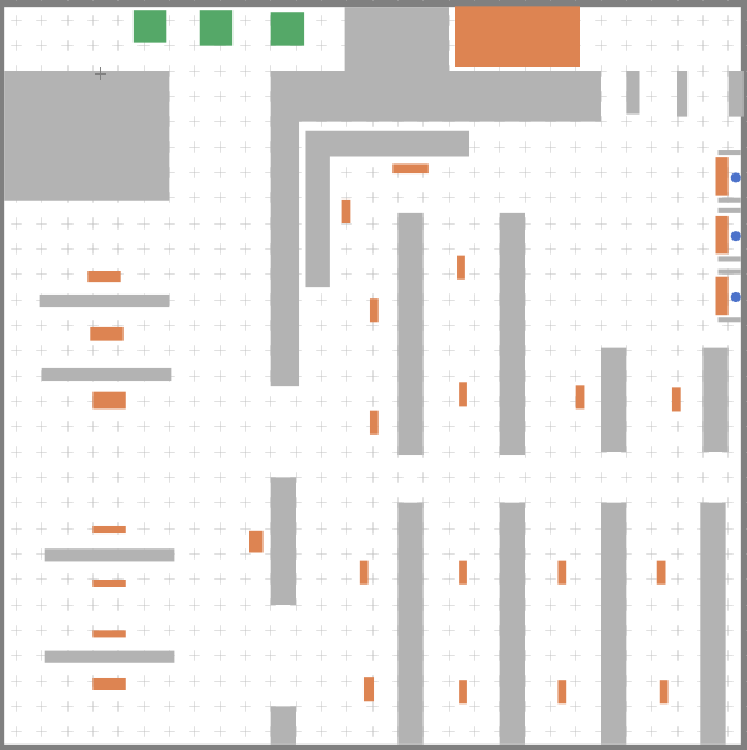
\includegraphics[width=0.4\textwidth]{images/5.3/supermarket.png}}
    \hfill
    \subfloat[b]{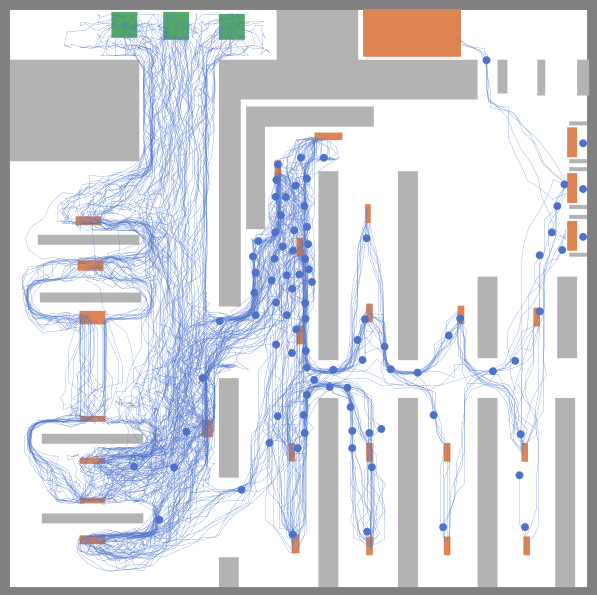
\includegraphics[width=0.4\textwidth]{images/5.3/crowded_moment.png}}
    \caption{On the left the supermarket scenario, on the right a depiction of a possible crowded moment}
    \label{fig:intro-supermarket}
\end{figure}

Making the scenario as realistic as possible is fundamental for a meaningful test. The pedestrian sources have been modified in their standard parameters so that they spawn pedestrians in groups of \textbf{3} for a certain time period (the first \textbf{150} seconds out of the total \textbf{400} simulated) following a spawning probability dictated by the \texttt{NegativeExponentialDistribution} parameter value. This was done to assure that not all pedestrians are spawned immediately (customers do not enter all at once in the supermarket, except for the American Black Friday), but that instead there is a continuous flow into the supermarket, not too empty and not too hectic, as a normal day would be. 

To make the scenario more realistic the three sources have been given three different routes to take, visiting some aisles and then going to one of the cash desks (where the cashiers are on the top right). They finally end their shopping by exiting through the bigger target on top. This was done to assure not all pedestrians follow the unrealistic rule of having the same exact supermarket route.

Two different tests are proposed in the following paragraphs:
\begin{itemize}
    \item \textbf{TEST A: }a scenario where the disease is not highly infective (\textbf{infectionRate: 0.02}) and the recovery rate is fairly low (\textbf{recoveryRate: 0.001}, more improbable, it would in fact be a very strange disease if in the course of a single shopping trip people get both infected and cured). The analysis shows the differences if no regulation on interpersonal distance is applied vs if \textbf{2.0} meters have to be kept between pedestrians when possible (as happened for a certain period in the current pandemic in Italy).
    \item \textbf{TEST B: }a scenario with a much more infective disease (\textbf{infectionRate: 0.10}) and the same recovery rate. The analysis shows how in such a scenario the social distancing is not enough because of the presence of bottlenecks in the supermarket, asking also for an entrance flow management (e.g. changing the spawned pedestrians per source from \textbf{3} to \textbf{2}).
\end{itemize}

Regarding TEST A, \textbf{\hyperref[fig:5.3-1.1]{Figure \ref{fig:5.3-1.1}}} shows the development of the simulation through some snapshots. As a reminder the simulation has the following parameters:
\begin{itemize}
    \item \textbf{infectionsAtStart:} 5
    \item \textbf{infectionRate:} 0.02
    \item \textbf{infectionMaxDistance:} 1.0
    \item \textbf{recoveryRate:} 0.001
    \item \textbf{pedPotentialPersonalSpaceWidth:} 0.9
    \item \textbf{pedestrians per source per spawning:} 3
\end{itemize}
The simulation shows how the infection spreads quite fast among the customers, with the infected being able to exploit the gathering shown in \textbf{\hyperref[fig:5.3-1.1]{Figure \ref{fig:5.3-1.1} (a) and (b)}}.
The infectivity of the disease is not too high and therefore not all customers get infected.

\begin{figure}[H]
    \centering
    \subfloat[a]{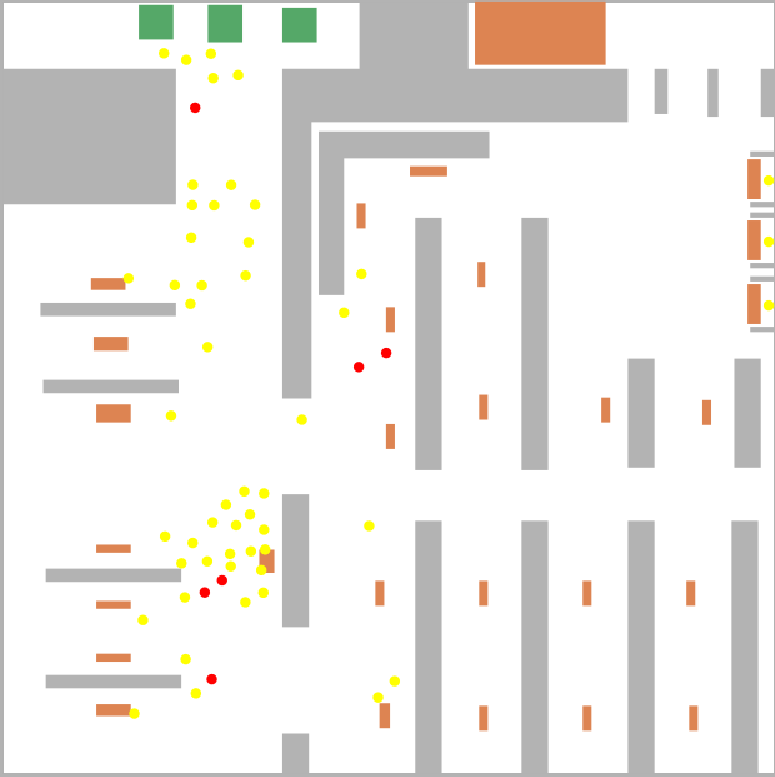
\includegraphics[width=0.3\textwidth]{images/5.3/1init.png}}
    \hfill
    \subfloat[b]{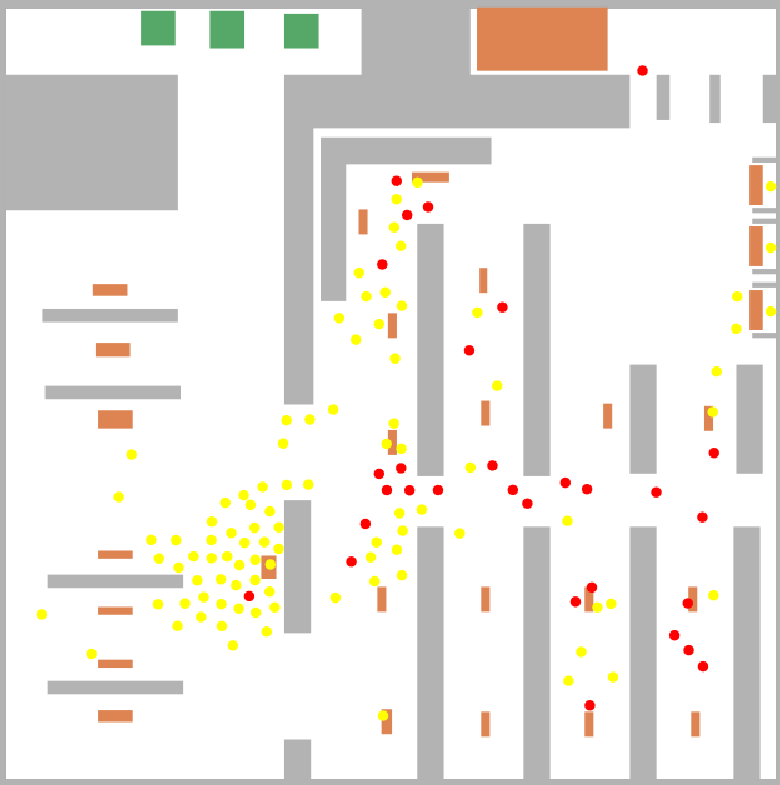
\includegraphics[width=0.3\textwidth]{images/5.3/1mid.png}}
    \hfill
    \subfloat[c]{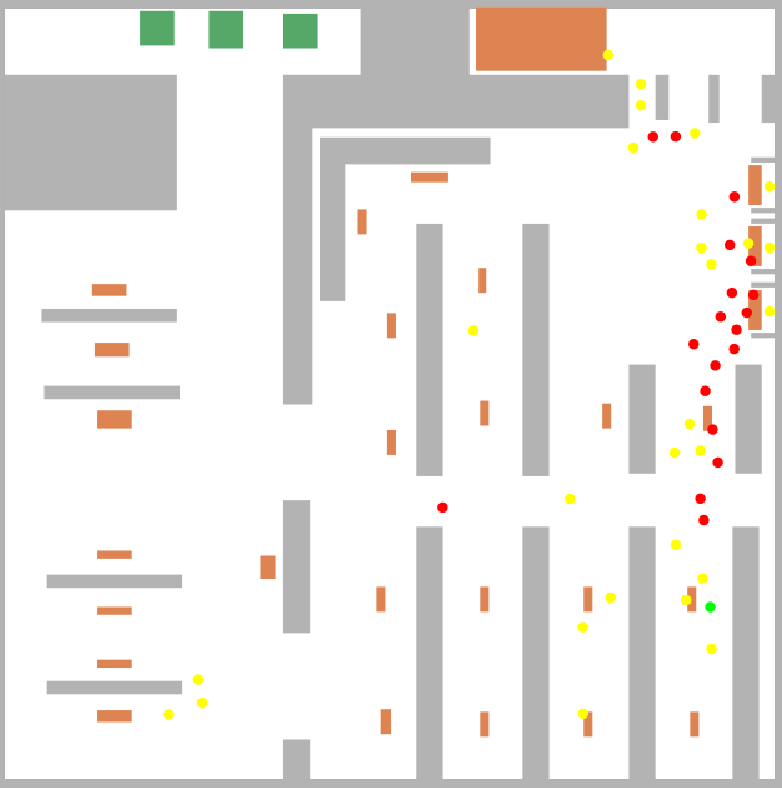
\includegraphics[width=0.3\textwidth]{images/5.3/1end.png}}
    \caption{Screenshots taken from the first test, having a \textbf{0.9} interpersonal space}
    \label{fig:5.3-1.1}
\end{figure}

A solution to the infective behaviour stands in applying some rules we are nowadays used to, for example \textit{Social Distancing}. What is shown in  \textbf{\hyperref[fig:5.3-1.2]{Figure \ref{fig:5.3-1.2}}} is the development of a comparative simulation where the parameters are:
\begin{itemize}
    \item \textbf{infectionsAtStart:} 5
    \item \textbf{infectionRate:} 0.02
    \item \textbf{infectionMaxDistance:} 1.0
    \item \textbf{recoveryRate:} 0.001
    \item \textbf{pedPotentialPersonalSpaceWidth:} \textbf{2.0}
    \item \textbf{pedestrians per source per spawning:} 3
\end{itemize}
Therefore one can notice how only the personal space width has changed, forcing the pedestrians to keep their distances when possible. The effect can be visually appreciated, with the infections being drastically reduced, showing the effectiveness of this approach.

\begin{figure}[H]
    \centering
    \subfloat[a]{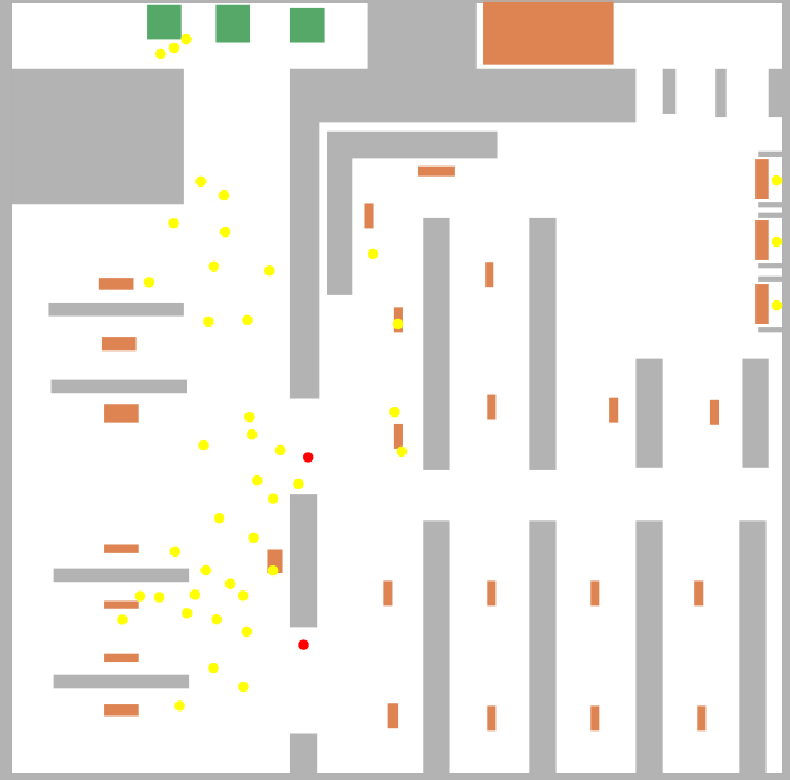
\includegraphics[width=0.3\textwidth]{images/5.3/2init.png}}
    \hfill
    \subfloat[b]{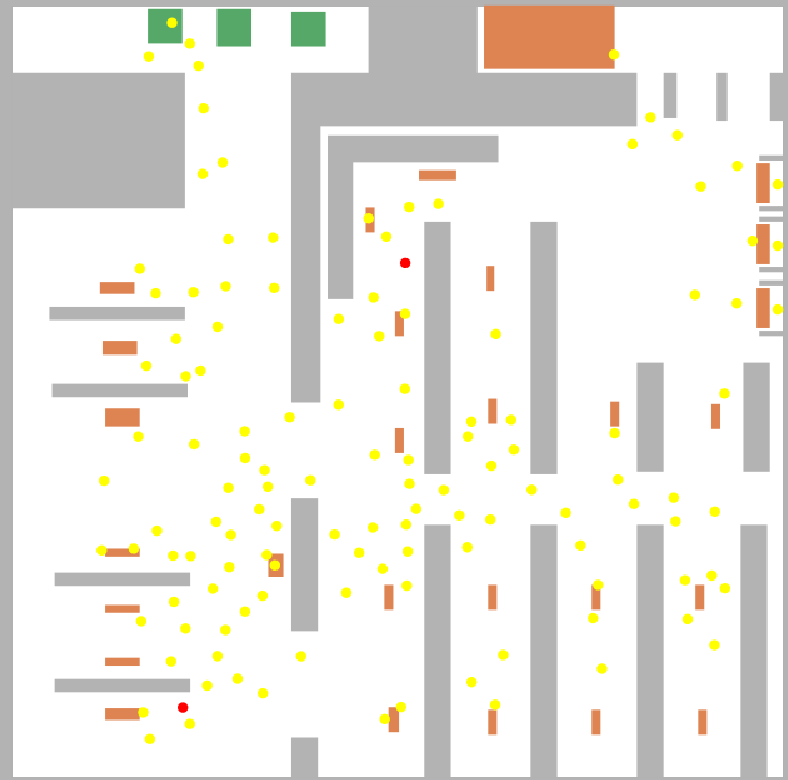
\includegraphics[width=0.3\textwidth]{images/5.3/2mid.png}}
    \hfill
    \subfloat[c]{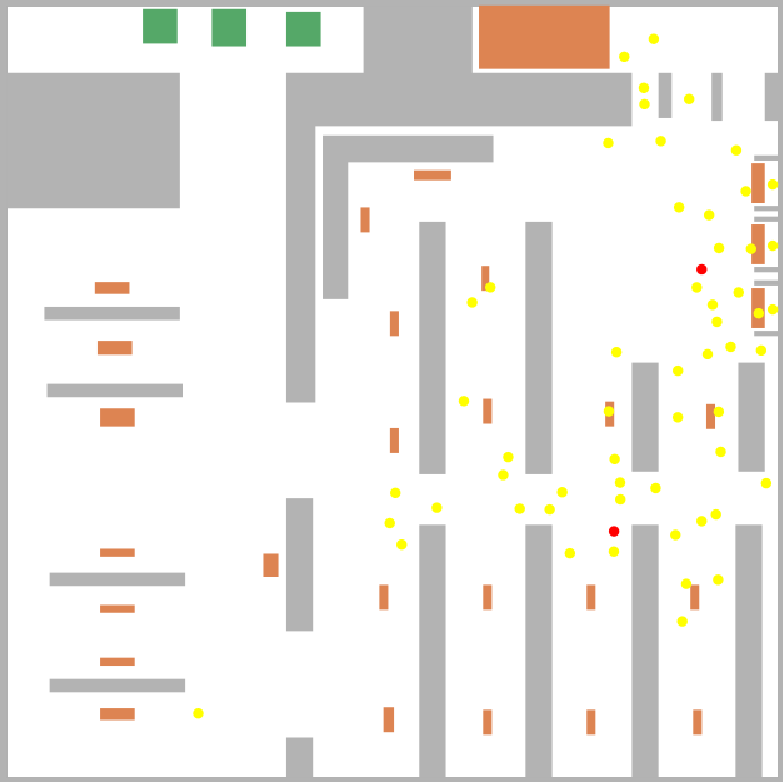
\includegraphics[width=0.3\textwidth]{images/5.3/2end.png}}
    \caption{Screenshots taken from the first test, having a \textbf{2.0} interpersonal space}
    \label{fig:5.3-1.2}
\end{figure}

Eventually, in \textbf{\hyperref[fig:first-test-dash]{Figure \ref{fig:first-test-dash}}}, a graphical comparison between the two simulations for TEST A is shown through \textit{Dash/Plotly}. In particular \texttt{test\_1\_1} represents the first simulation and \texttt{test\_1\_2} the second one, remarking again the effectiveness of increasing the social distancing in having less infections.

\begin{figure}[H]
    \centering
    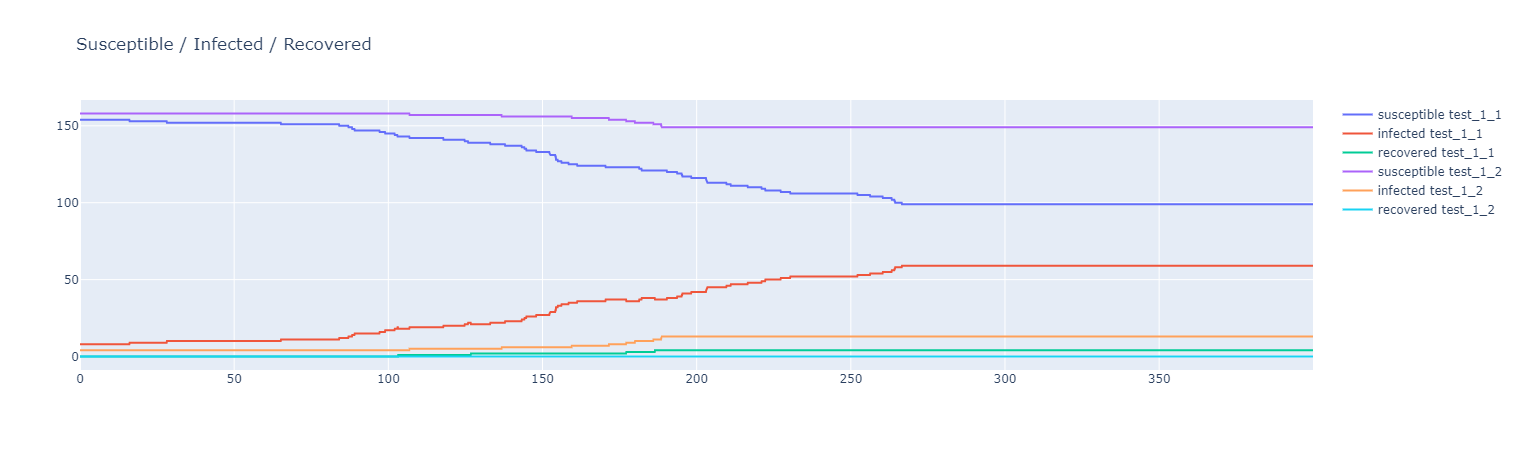
\includegraphics[scale=0.3]{images/5.3/first_test_dash.png}
    \caption{Graphic visualization using \textit{Dash/Plotly} of the first test}
    \label{fig:first-test-dash}
\end{figure}

Moving on to TEST B, a different scenario is portrayed. Here a much higher infection rate is present, causing the social distancing to be less efficient. The test proposes a change in the entry flow of the supermarket which in combination with social distancing proves to be working better.
\textbf{\hyperref[fig:5.3-2.1]{Figure \ref{fig:5.3-2.1}}} refers to the TEST B scenario where no precautions are taken into consideration. The simulation parameters are:
\begin{itemize}
    \item \textbf{infectionsAtStart:} 0
    \item \textbf{infectionRate:} 0.10
    \item \textbf{infectionMaxDistance:} 1.0
    \item \textbf{recoveryRate:} 0.001
    \item \textbf{pedPotentialPersonalSpaceWidth:} \textbf{1.0}
    \item \textbf{pedestrians per source per spawning:} 3
\end{itemize}
The simulation shows how the infection spreads incredibly fast among the customers, reaching almost all the customers and also infecting one of the poor cashiers. The higher number of infected in this experiment gives rise also to some recovered popping up somewhere in the simulation. One example is the cashier who has a miracolous infection and recovery during a single working shift, impressive!\\
Such a situation should not happen and this leads to the second part of the TEST B.

\begin{figure}[H]
    \centering
    \subfloat[a]{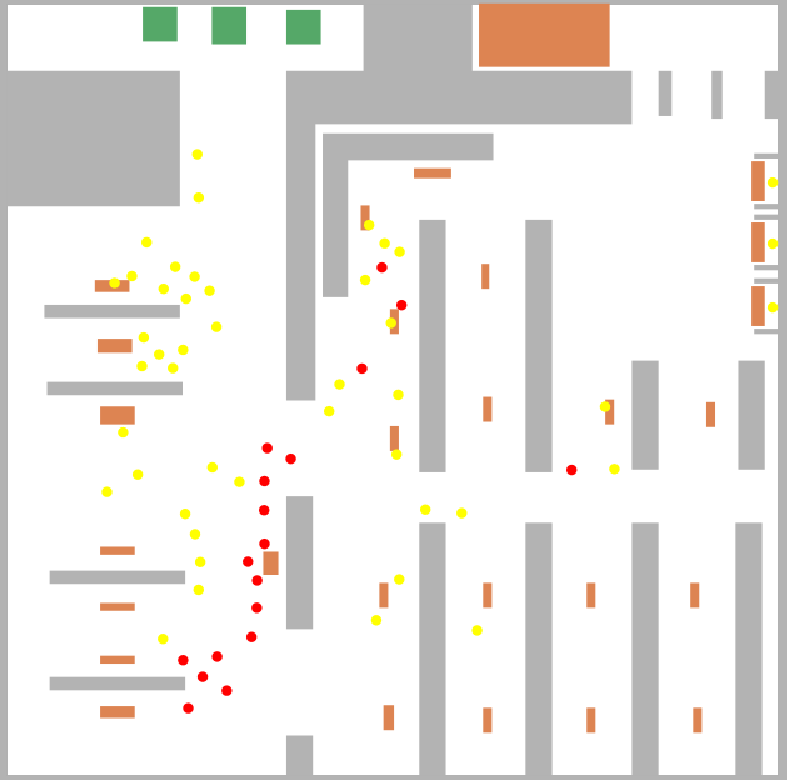
\includegraphics[width=0.3\textwidth]{images/5.3/3init.png}}
    \hfill
    \subfloat[b]{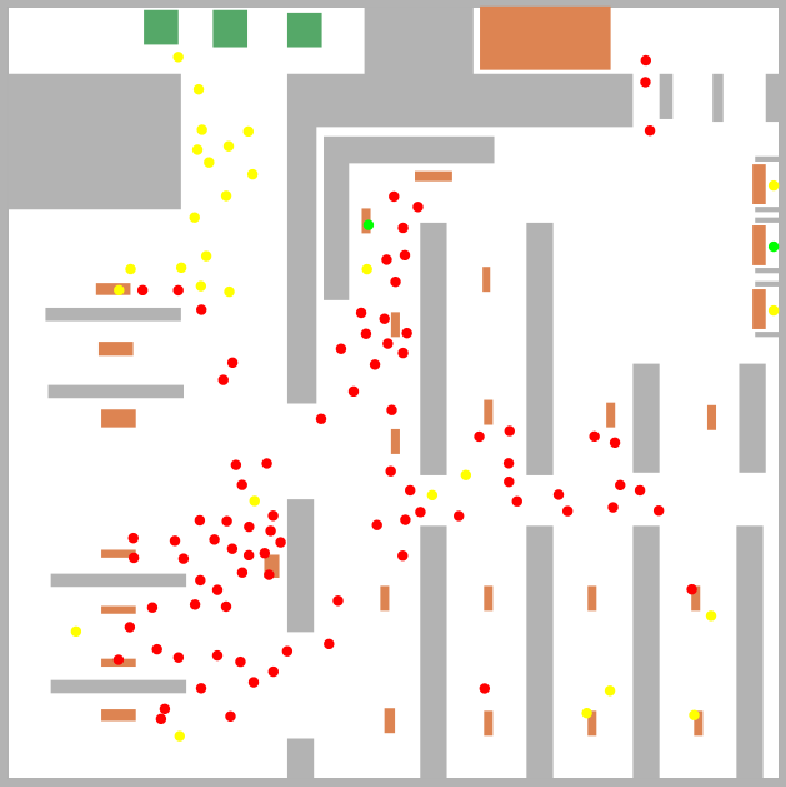
\includegraphics[width=0.3\textwidth]{images/5.3/3mid.png}}
    \hfill
    \subfloat[c]{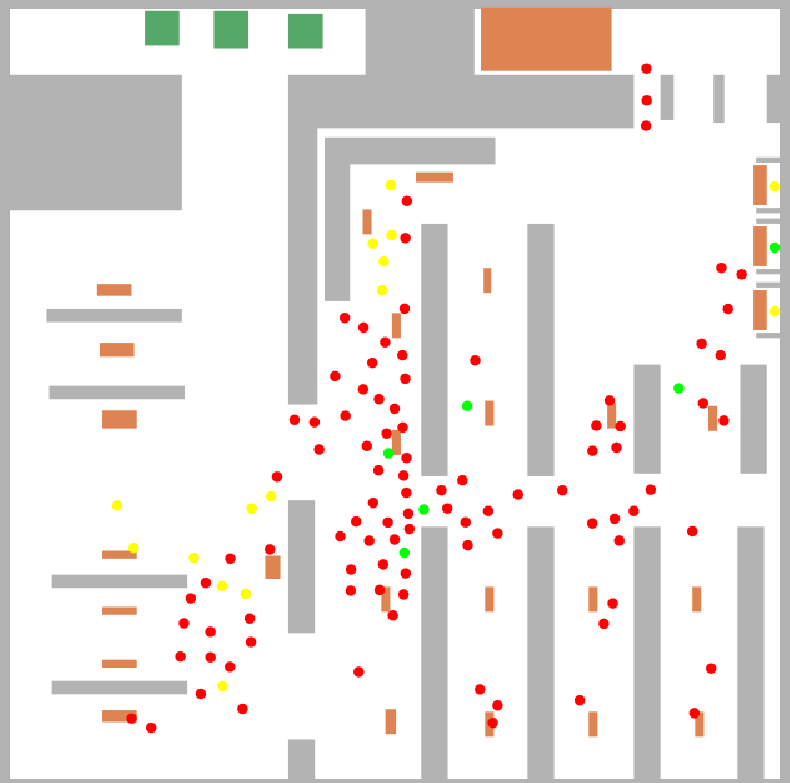
\includegraphics[width=0.3\textwidth]{images/5.3/3end.png}}
    \caption{Screenshots taken from the second test, having a \textbf{1.0} interpersonal space}
    \label{fig:5.3-2.1}
\end{figure}

A possible mitigation of the infective behaviour stands in applying as previously mentioned some rules. What is shown in  \textbf{\hyperref[fig:5.3-1.2]{Figure \ref{fig:5.3-1.2}}} is the development of a comparative simulation where the parameters are:
\begin{itemize}
    \item \textbf{infectionsAtStart:} 0
    \item \textbf{infectionRate:} 0.1
    \item \textbf{infectionMaxDistance:} 1.0
    \item \textbf{recoveryRate:} 0.001
    \item \textbf{pedPotentialPersonalSpaceWidth:} \textbf{2.0}
    \item \textbf{pedestrians per source per spawning:} 2
\end{itemize}
It is possible to notice how the combination of both a higher inter-person space and a slower entrance flow gives a considerably better result, with littler infections. It is interesting to notice that infections are anyhow existent. This is due to the higher infection rate: if the infection rate is high it is possible to get infected even in a smaller gathering time window, well simulating a more aggressive disease. The responsibility is not only on that argument, but also partly on Vadere: the software simulation has the chance to spawn infected pedestrians, and having a higher infection rate helps this process.

\begin{figure}[H]
    \centering
    \subfloat[a]{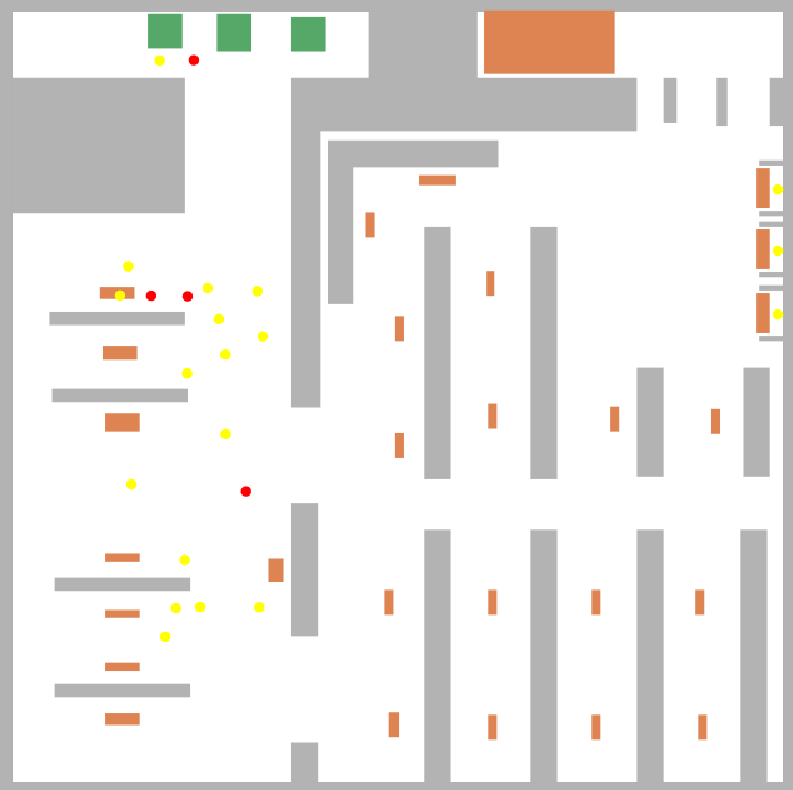
\includegraphics[width=0.3\textwidth]{images/5.3/4init.png}}
    \hfill
    \subfloat[b]{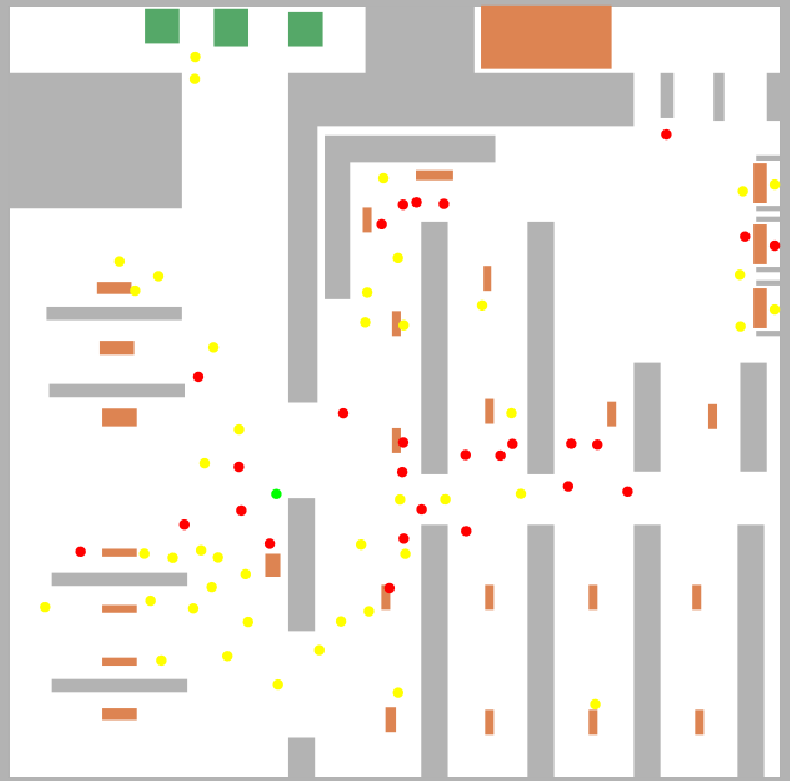
\includegraphics[width=0.3\textwidth]{images/5.3/4mid.png}}
    \hfill
    \subfloat[c]{\includegraphics[width=0.3\textwidth]{images/5.3/4end.png}}
    \caption{Screenshots taken from the second test, having a \textbf{2.0} interpersonal space and lower entrance rate}
    \label{fig:5.3-2.2}
\end{figure}

Finally, as for the TEST A, a \textit{Dash/Plotly} graphic in \textbf{\hyperref[fig:second-test-dash]{Figure \ref{fig:second-test-dash}}} is shown to better portray the comparison. In particular \texttt{test\_2\_1} represents the first simulation and \texttt{test\_2\_2} the second one.\\
It is important to remark that the simulation where all precautions are taken into consideration effectively spawns a lower amount of pedestrians (lower entrance flow, same execution time), therefore the plot has to be analyzed with that in mind. The graphic does nevertheless show how a combination of precautions does help the decrease in spreading even against a more aggressive disease.
\begin{figure}[H]
    \centering
    \includegraphics[scale=0.3]{images/5.3/second_test_dash.png}
    \caption{Graphic visualization using \textit{Dash/Plotly} of the second test}
    \label{fig:second-test-dash}
\end{figure}

\end{task}

\newpage
\bibliographystyle{plain}
\bibliography{Literature}

\end{document}